\documentclass[12pt, a4paper]{article}

%<*preamble>
% Math symbols
\usepackage{amsmath, amsthm, amsfonts, amssymb}
\usepackage{accents}
\usepackage{esvect}
\usepackage{mathrsfs}
\usepackage{mathtools}
\mathtoolsset{showonlyrefs}
\usepackage{cmll}
\usepackage{stmaryrd}
\usepackage{physics}
\usepackage[normalem]{ulem}
\usepackage{ebproof}
\usepackage{extarrows}

% Page layout
\usepackage{geometry, a4wide, parskip, fancyhdr}

% Font, encoding, russian support
\usepackage[russian]{babel}
\usepackage[sb]{libertine}
\usepackage{xltxtra}

% Listings
\usepackage{listings}
\lstset{basicstyle=\ttfamily,breaklines=true}
\setmonofont{Inconsolata}

% Miscellaneous
\usepackage{array}
\usepackage{calc}
\usepackage{caption}
\usepackage{subcaption}
\captionsetup{justification=centering,margin=2cm}
\usepackage{catchfilebetweentags}
\usepackage{enumitem}
\usepackage{etoolbox}
\usepackage{float}
\usepackage{lastpage}
\usepackage{minted}
\usepackage{svg}
\usepackage{wrapfig}
\usepackage{xcolor}
\usepackage[makeroom]{cancel}

\newcolumntype{L}{>{$}l<{$}}
    \newcolumntype{C}{>{$}c<{$}}
\newcolumntype{R}{>{$}r<{$}}

% Footnotes
\usepackage[hang]{footmisc}
\setlength{\footnotemargin}{2mm}
\makeatletter
\def\blfootnote{\gdef\@thefnmark{}\@footnotetext}
\makeatother

% References
\usepackage{hyperref}
\hypersetup{
    colorlinks,
    linkcolor={blue!80!black},
    citecolor={blue!80!black},
    urlcolor={blue!80!black},
}

% tikz
\usepackage{tikz}
\usepackage{tikz-cd}
\usetikzlibrary{arrows.meta}
\usetikzlibrary{decorations.pathmorphing}
\usetikzlibrary{calc}
\usetikzlibrary{patterns}
\usepackage{pgfplots}
\pgfplotsset{width=10cm,compat=1.9}
\newcommand\irregularcircle[2]{% radius, irregularity
    \pgfextra {\pgfmathsetmacro\len{(#1)+rand*(#2)}}
    +(0:\len pt)
    \foreach \a in {10,20,...,350}{
            \pgfextra {\pgfmathsetmacro\len{(#1)+rand*(#2)}}
            -- +(\a:\len pt)
        } -- cycle
}

\providetoggle{useproofs}
\settoggle{useproofs}{false}

\pagestyle{fancy}
\lfoot{M3137y2019}
\cfoot{}
\rhead{стр. \thepage\ из \pageref*{LastPage}}

\newcommand{\R}{\mathbb{R}}
\newcommand{\Q}{\mathbb{Q}}
\newcommand{\Z}{\mathbb{Z}}
\newcommand{\B}{\mathbb{B}}
\newcommand{\N}{\mathbb{N}}
\renewcommand{\Re}{\mathfrak{R}}
\renewcommand{\Im}{\mathfrak{I}}

\newcommand{\const}{\text{const}}
\newcommand{\cond}{\text{cond}}

\newcommand{\teormin}{\textcolor{red}{!}\ }

\DeclareMathOperator*{\xor}{\oplus}
\DeclareMathOperator*{\equ}{\sim}
\DeclareMathOperator{\sign}{\text{sign}}
\DeclareMathOperator{\Sym}{\text{Sym}}
\DeclareMathOperator{\Asym}{\text{Asym}}

\DeclarePairedDelimiter{\ceil}{\lceil}{\rceil}

% godel
\newbox\gnBoxA
\newdimen\gnCornerHgt
\setbox\gnBoxA=\hbox{$\ulcorner$}
\global\gnCornerHgt=\ht\gnBoxA
\newdimen\gnArgHgt
\def\godel #1{%
    \setbox\gnBoxA=\hbox{$#1$}%
    \gnArgHgt=\ht\gnBoxA%
    \ifnum     \gnArgHgt<\gnCornerHgt \gnArgHgt=0pt%
    \else \advance \gnArgHgt by -\gnCornerHgt%
    \fi \raise\gnArgHgt\hbox{$\ulcorner$} \box\gnBoxA %
    \raise\gnArgHgt\hbox{$\urcorner$}}

% \theoremstyle{plain}

\theoremstyle{definition}
\newtheorem{theorem}{Теорема}
\newtheorem*{definition}{Определение}
\newtheorem{axiom}{Аксиома}
\newtheorem*{axiom*}{Аксиома}
\newtheorem{lemma}{Лемма}

\theoremstyle{remark}
\newtheorem*{remark}{Примечание}
\newtheorem*{exercise}{Упражнение}
\newtheorem{corollary}{Следствие}[theorem]
\newtheorem*{statement}{Утверждение}
\newtheorem*{corollary*}{Следствие}
\newtheorem*{example}{Пример}
\newtheorem{observation}{Наблюдение}
\newtheorem*{prop}{Свойства}
\newtheorem*{obozn}{Обозначение}

% subtheorem
\makeatletter
\newenvironment{subtheorem}[1]{%
    \def\subtheoremcounter{#1}%
    \refstepcounter{#1}%
    \protected@edef\theparentnumber{\csname the#1\endcsname}%
    \setcounter{parentnumber}{\value{#1}}%
    \setcounter{#1}{0}%
    \expandafter\def\csname the#1\endcsname{\theparentnumber.\Alph{#1}}%
    \ignorespaces
}{%
    \setcounter{\subtheoremcounter}{\value{parentnumber}}%
    \ignorespacesafterend
}
\makeatother
\newcounter{parentnumber}

\newtheorem{manualtheoreminner}{Теорема}
\newenvironment{manualtheorem}[1]{%
    \renewcommand\themanualtheoreminner{#1}%
    \manualtheoreminner
}{\endmanualtheoreminner}

\newcommand{\dbltilde}[1]{\accentset{\approx}{#1}}
\newcommand{\intt}{\int\!}

% magical thing that fixes paragraphs
\makeatletter
\patchcmd{\CatchFBT@Fin@l}{\endlinechar\m@ne}{}
{}{\typeout{Unsuccessful patch!}}
\makeatother

\newcommand{\get}[2]{
    \ExecuteMetaData[#1]{#2}
}

\newcommand{\getproof}[2]{
    \iftoggle{useproofs}{\ExecuteMetaData[#1]{#2proof}}{}
}

\newcommand{\getwithproof}[2]{
    \get{#1}{#2}
    \getproof{#1}{#2}
}

\newcommand{\import}[3]{
    \subsection{#1}
    \getwithproof{#2}{#3}
}

\newcommand{\given}[1]{
    Дано выше. (\ref{#1}, стр. \pageref{#1})
}

\renewcommand{\ker}{\text{Ker }}
\newcommand{\im}{\text{Im }}
\renewcommand{\grad}{\text{grad}}
\newcommand{\rg}{\text{rg}}
\newcommand{\defeq}{\stackrel{\text{def}}{=}}
\newcommand{\defeqfor}[1]{\stackrel{\text{def } #1}{=}}
\newcommand{\itemfix}{\leavevmode\makeatletter\makeatother}
\newcommand{\?}{\textcolor{red}{???}}
\renewcommand{\emptyset}{\varnothing}
\newcommand{\longarrow}[1]{\xRightarrow[#1]{\qquad}}
\DeclareMathOperator*{\esup}{\text{ess sup}}
\newcommand\smallO{
    \mathchoice
    {{\scriptstyle\mathcal{O}}}% \displaystyle
    {{\scriptstyle\mathcal{O}}}% \textstyle
    {{\scriptscriptstyle\mathcal{O}}}% \scriptstyle
    {\scalebox{.6}{$\scriptscriptstyle\mathcal{O}$}}%\scriptscriptstyle
}
\renewcommand{\div}{\text{div}\ }
\newcommand{\rot}{\text{rot}\ }
\newcommand{\cov}{\text{cov}}

\makeatletter
\newcommand{\oplabel}[1]{\refstepcounter{equation}(\theequation\ltx@label{#1})}
\makeatother

\newcommand{\symref}[2]{\stackrel{\oplabel{#1}}{#2}}
\newcommand{\symrefeq}[1]{\symref{#1}{=}}

% xrightrightarrows
\makeatletter
\newcommand*{\relrelbarsep}{.386ex}
\newcommand*{\relrelbar}{%
    \mathrel{%
        \mathpalette\@relrelbar\relrelbarsep
    }%
}
\newcommand*{\@relrelbar}[2]{%
    \raise#2\hbox to 0pt{$\m@th#1\relbar$\hss}%
    \lower#2\hbox{$\m@th#1\relbar$}%
}
\providecommand*{\rightrightarrowsfill@}{%
    \arrowfill@\relrelbar\relrelbar\rightrightarrows
}
\providecommand*{\leftleftarrowsfill@}{%
    \arrowfill@\leftleftarrows\relrelbar\relrelbar
}
\providecommand*{\xrightrightarrows}[2][]{%
    \ext@arrow 0359\rightrightarrowsfill@{#1}{#2}%
}
\providecommand*{\xleftleftarrows}[2][]{%
    \ext@arrow 3095\leftleftarrowsfill@{#1}{#2}%
}

\allowdisplaybreaks

\newcommand{\unfinished}{\textcolor{red}{Не дописано}}

% Reproducible pdf builds 
\special{pdf:trailerid [
<00112233445566778899aabbccddeeff>
<00112233445566778899aabbccddeeff>
]}
%</preamble>


\lhead{Дифференциальные уравнения}
\cfoot{}
\rfoot{Конспект к экзамену}

\usepackage{graphicx}

\newcommand{\tr}{\text{tr}}

\begin{document}

\section*{Основные вопросы}

\subsection*{1. Уравнение с разделяющимися переменными: общее решение, общая схема исследования.}

Уравнение с \textbf{разделенными} переменными имеет вид:
\[X(x)dx + Y(y)dy = 0\]

У него решение имеет вид:
\[\int X(x) dx + \int Y(y)dy = C\]

\begin{proof}
    \[\int X(x) dx + \int Y(y)dy = \int X(x) dx + \int Y(y)y' dx = \int (X(x) + Y(y)y')dx = \int 0dx = C\]
\end{proof}

При этом мы получаем общее решение, когда находим такие \(C\), что ответ \(\in C^1\).

Уравнение с \textbf{разделяющимися} переменными имеет вид:
\[p_1(x)q_1(y)dx + p_2(x)q_2(y)dy = 0\]

Если поделить на \(p_2(x)q_1(y)\), то получим уравнение с разделенными переменными. При этом необходимо убедиться, что мы не делим на ноль.

Если \(\exists y_0 : q_1(y_0) = 0\), то \(y\equiv y_0\) --- решение исходного уравнения. Исключив \(y_0\), мы разбиваем область возможных решений на две подобласти.

Аналогично для \(x\).

После разбиения нужно на каждой области найти решение.

\subsection*{2. Линейное уравнение 1-го порядка: общее решение ЛОУ, общее решение ЛНУ. Метод Лагранжа и метод интегрирующего множителя.}

Линейное уравнение первого порядка это
\[y' = p(x)y + q(x)\]

Если \(q\equiv 0\), то это уравнение \textbf{однородно}, иначе \textbf{неоднородно}.

Общее решение ЛОУ это \(y = Ce^{\int p}, C\in\R\)

\begin{proof}
    Заметим, что \(y\equiv 0\) --- решение. По теореме о единственности оно не является особым. т.к. мы рассматриваем \(p\in C(a, b)\).

    \(\sphericalangle y > 0\).
    \[\frac{dy}{y} = p(x)dx\]
    \[\ln y = \int p(x)dx + C\]
    \[y = e^C e^{\int p(x)dx}\]
    По теореме об общем решении уравнения с разделенными переменными это семейство всех решений исходного уравнения при \(y > 0\).

    Аналогично при \(y < 0\)
\end{proof}

Общее решение ЛНУ это
\[y = \left( C + \int qe^{ -\int p} \right)e^{\int p}\]
\begin{proof}
    Подстановкой легко показать, что это решение. Покажем, что нет других решений.

    Пусть есть решение \(\varphi\) на \((\alpha, \beta)\), не подходящее под искомую формулу.

    Пусть \(x_0 \in (\alpha,\beta)\) и \(\varphi(x_0) = y_0\).

    Функция
    \[C = \left( y_0 e^{ -\int p} - \int q e^{ -\int p} dx\right)\Bigg|_{x = x_0}\]

    подходит под искомую формулу, но при этом является решением задачи Коши \(y(x_0) = y_0\), поэтому \(y \equiv \varphi\) --- противоречие.
\end{proof}

\textbf{Метод Лагранжа \textit{(вариации произвольной постоянной)}} --- постоянную \(C\) считают функцией от \(x\) и получают дифур относительно \(C\).

\subsection*{3. Равностепенно непрерывные функции. Лемма Арцела–Асколи.}

Множество функций \(F \), определенных на \(D\), \textbf{равностепенно непрерывно}, если:
\[\forall \varepsilon > 0 \ \ \exists \delta > 0 \ \ \forall f\in F \ \ \forall x_1, x_2\in D \ \ |x_2 - x_1|< \delta \Rightarrow |f(x_2) - f(x_1)|< \varepsilon\]

\begin{lemma}
    Пусть функции последовательности \(\{f_n\}_{n = 1}^{\infty}\) равномерно ограничены \textit{(\(\exists C : \forall n, x |f_n(x)| < C\))} и равностепенно непрерывны на \([a, b]\). Тогда из нее можно выделить подпоследовательность, равномерно сходящуюся на \([a, b]\).
\end{lemma}
\begin{proof}
    Пусть \(M\) ограничивает \textit{(равномерно)} \(f_n\):
    \[M : = \sup_{n, x} |f_n(x)|\]
    \[\sphericalangle \varepsilon_k = \frac{M}{2^{k + 1}}\]
    \[\forall \varepsilon_k > 0 \ \ \exists \delta_k > 0 \ \ \forall f\in F \ \ \forall x_1, x_2\in D \ \ |x_2 - x_1|< \delta_k \Rightarrow |f(x_2) - f(x_1)|< \varepsilon_k\]

    Поделим всю область \([a, b] \times ( - M, M)\) на прямоугольники со стороной \(\varepsilon_1\) и \(\delta_1\).

    Рассмотрим первый столбец. Возьмём два произвольных соседних прямоугольника, таких что по ним проходит бесконечное число \(f\). Вырежем все \(f\), которые по этим прямоугольникам не подходят. Сделаем то же самое для каждого столбца. Получим в итоге \textit{(бесконечную)} подпоследовательность \(F^*_1\).

    Повторим то же самое для всех \(\varepsilon_n, \delta_n\).

    \[\forall f, g\in F^*_i \ \ \forall x\in[a, b] \ \ |f(x) - g(x)| < 2 \varepsilon_n\]
    Нам нужно показать, что \(\forall \varepsilon > 0 \ \ \forall N, k \ \ \forall x\in[a, b] \ \ |f^*_N(x) - f^*_{N + k}(x)|< \varepsilon\)

    Тогда возьмём \(N : 2 \varepsilon_N < \varepsilon\) и все получится, т.к. \(F^*_N \supset F^*_{N + k}\)
\end{proof}

\subsection*{4. ЗК для нормальной системы. Лемма о равносильном интегральном уравнении. Лемма: свойства ломаной Эйлера, определённой на отрезке Пеано.}

Задача Коши для нормальной системы --- нахождение решения, подходящего под условие \(r(t_0) = r_0\)

\(f : \R^{n + 1} \to \R^n\), тогда \(\varphi\) --- решение на \([a, b]\) интегрального уравнения
\[r(t) = r_0 + \int_{t_0}^t f(\tau, r(\tau)) d\tau\]
, если:
\begin{enumerate}
    \item \(\varphi\in C([a, b] \to \R^n)\)
    \item \(\varphi(t) \equiv r_0 + \int_{t_0}^{t} f(\tau, \varphi(\tau)) d\tau\) на \([a, b]\)
\end{enumerate}

\begin{lemma}
    \(\varphi\) --- решение задачи Коши \(\dot r = f(t, r), r\) эквивалентно тому, что \(\varphi\) --- решение
    \[r(t) = r_0 + \int_{t_0}^t f(\tau, r(\tau)) d\tau\]
\end{lemma}
\begin{proof}\itemfix
    \begin{itemize}
        \item [\( \Rightarrow \)] Проинтегрируем \(\dot \varphi(t) = f(\tau, \varphi(\tau))\) от \(t_0\) до \(t\)
        \item [\( \Leftarrow \)] Продифференцируем интегральное уравнение.
    \end{itemize}
\end{proof}

\begin{definition}[Отрезок Пеано]
    \(G\subset \R^{n + 1}_{t, r}\) --- область, \((t_0, r_0)\in G\). Т.к. \(G\) открыто, \(\exists a, b > 0\), такие что параллелепипед с центром в \((t_0, r_0)\) и сторонами \(a, b\) (\(|t - t_0| \leq a, |r - r_0| \leq b\)) лежит в \(G\).

    По теореме Вейерштрасса на компакте есть максимум, т.е. \(\exists M = \max\limits_{\Pi} |f|\). Пусть \(h = \min \{a, \frac{b}{M}\} \). Тогда отрезок \([t_0 - h, t_0 + h]\) --- \textbf{отрезок Пеано}
\end{definition}

Рассмотрим некоторый отрезок Пеано и поделим его правую часть на \(N\) равных частей точками \(t_k\).

Пусть ломаная Эйлера \(E_N\) определена рекурсивно:
\begin{enumerate}
    \item \(E_N(t_0) = r_0\)
    \item \(E_N(t) = E_N(t_k) + f(t_k, E_N(t_k))(t - t_k)\), если \(t\in(t_k, t_{k+1}]\)
\end{enumerate}

\begin{lemma}
    \(\forall t\in[t_0, t_0 + h]\):
    \begin{enumerate}
        \item \(\exists E_N(t)\)
        \item \(|E_N(t) - r_0| \leq M(t - t_0)\), т.е. оно лежит в треугольнике.
    \end{enumerate}
\end{lemma}
\begin{proof}
    Докажем по индукции, что это верно при \(t\in[t_0, t_k]\) для всех \(k\).

    При \(k = 1\) \(E_N\) действительно определена, т.к. \(E_N(t) = r_0 + f(t_0, r_0)(t - t_0)\)

    \[|E_N(t) - r_0| = |f(t_0, r_0)(t - t_0)| \leq M(t - t_0)\]

    Переход индукции:
    \[|E_N(t_k) - r_0| \leq M(t_k - t_0) \leq Mh \leq M \frac{b}{M} = b\]
    Таким образом мы лежим в \(\Pi\), все определено.

    \[|E_N(t) - r_0| = |E_N(t) - E_N(t_0)| \leq |E_N(t) - E_N(t_0)| + |E_N(t_k) - E_N(t_0)| \leq\]
    \[|f(t_k, E_N(t_k))|(t - t_k) + M(t_k - t_0) \leq M(t - t_k) + M(t_k - t_0) = M(t - t_0)\]
\end{proof}

\subsection*{5. Теорема Пеано о существовании решения ЗК.}

\begin{theorem}
    \(G\subset \R^{n + 1}_{t, r}\) --- область, \(f\in C(G\to\R^n), (t_0, r_0)\in G\). Тогда задача Коши имеет решение, определенное на отрезке Пеано для \((t_0, r_0)\).
\end{theorem}
\begin{proof}
    Пусть \(t_0 = 0, r_0 = 0\) \textit{(сдвиг координат)}. Пусть \([ - h, h]\) --- искомый отрезок Пеано. Докажем для \([0, h]\), для другой части аналогично. Объединить оба решения можно по лемме о гладкой стыковке решений.

    Построим бесконечную последовательность ломаных Эйлера. Мы знаем, что \(|E_N(t)| \leq b\), т.е. она равномерно ограничена.

    \[|E_N(t_2) - E_N(t_1)| = \left|\int_{t_1}^{t_2} \dot E_N(\tau)d\tau\right| \leq \int_{t_1}^{t_2} |\dot{E}_N(\tau)|dt\]
    Мы знаем, что \(|\dot{E}_N(t)| \leq M\), поэтому:
    \[|E_N(t_2) - E_N(t_1)| \leq \int_{t_1}^{t_2} |\dot{E}_N(\tau)|dt \leq M(t_2 - t_1)\]
    Пусть \(|t_2 - t_1|< \delta\), тогда \(|E_N(t_2) - E_N(t_1)| < M\delta\) и пусть \(\delta = \frac{\varepsilon}{M}\), тогда \(|E_N(t_2) - E_N(t_1)| < \varepsilon\), т.е. \(E_N\) равностепенно непрерывна. По лемме Арцела–Асколи у этой последовательности есть подпоследовательность, равномерно сходящаяся к некоторой функции \(\varphi\). Покажем, что \(\varphi\) --- решение задачи Коши. Для этого достаточно показать, что:
    \[\varphi(t) \equiv \int_0^{t} f(\tau, \varphi(\tau))d\tau \text{ на } [0, h]\]
    Пусть теперь \(E_N\) --- подпоследовательность исходной последовательности.

    По формуле Ньютона-Лейбница для отображений:
    \[E_N(t) = \int_0^t \dot{E}_N(\tau)d\tau\]
    \[\varphi(t) = \lim_{N \to +\infty}\int_0^t \dot{E}_N(\tau)d\tau\]
    Таким образом, надо показать, что
    \[\lim_{N \to +\infty}\int_0^t \dot{E}_N(\tau)d\tau = \int_0^{t} f(\tau, \varphi(\tau))d\tau\]
    Покажем, что
    \[\Delta_N = \left|\int_0^{t} f(\tau, \varphi(\tau))d\tau - \int_0^t \dot{E}_N(\tau)d\tau\right| \to 0\]
    \[\Delta_N \leq \int_0^t |\dot{E}_N(\tau) - f(\tau, \varphi(\tau))|d\tau \leq \int_0^h |\dot{E}_N(\tau) - f(\tau, \varphi(\tau))|d\tau =\]
    \[\sum_{k = 0}^{N - 1} \int_{t_k}^{t_{k+1}} |\dot{E}_N(\tau) - f(\tau, \varphi(\tau))|d\tau = \sum_{k = 0}^{N - 1} \int_{t_k}^{t_{k+1}} |f(t_k, E_N(t_k)) - f(\tau, \varphi(\tau))|d\tau\]
    \(f\) равномерно непрерывна на параллелепипеде, поэтому \(|(t_k, E_N(t_k)) - (\tau, \varphi(\tau))| < \delta \Rightarrow |f(t_k, E_N(t_k)) - f(\tau, \varphi(\tau))| < \varepsilon\)
    \[\int_{t_k}^{t_{k+1}} |f(t_k, E_N(t_k)) - f(\tau, \varphi(\tau))|d\tau < \varepsilon h\]
    Тогда по двойной бухгалтерии \(\Delta_N \to 0\).

    Но мы не доказали, что \(|(t_k, E_N(t_k)) - (\tau, \varphi(\tau))| < \delta\).

    \[|(t_k, E_N(t_k)) - (\tau, \varphi(\tau))| \leq |(t_k, E_N(t_k)) - (t_k, \varphi(t_k))| + |(t_k, \varphi(t_k)) - (\tau, \varphi(t_k))| + |(\tau, \varphi(t_k)) - (\tau, \varphi(\tau))|\]
    \[ = |E_N(t_k) - \varphi(t_k)| + |t_k - \tau| + |\varphi(t_k) - \varphi(\tau)|\]

    При достаточно больших \(N\) все три слагаемых \( < \frac{\delta}{3}\)
\end{proof}

\subsection*{6. Достаточное условие того, что функция удовлетворяет локальному условию Липшица по заданной переменной.}

Пусть \(G\subset \R^{n + 1}_{t, r}\) --- область, \(f\in C(G \to \R^n), f'_r \in M_{m,n}(C(G))\). Тогда \(f\in \text{Lip}_{r, loc}(G)\)

Кроме того, если \(K\subset G\) --- выпуклый компакт, то \(M_1 : = \max\limits_{(t, r)\in K}|f'_r(t, r)|\), то:
\[\forall (t, r_1), (t, r_2)\in K \ \ |f(t, r_2) - f(t, r_1)| \leq nM_1|r_2 - r_1|\]

\begin{proof}
    Докажем, что на выпуклом компакте \(f\in \text{Lip}_r(K)\).

    Зададим \(g(s) = f(t, r_1 + s(r_2 - r_1))\) \textit{(т.к. \(K\) выпуклый, функция везде определена)}

    \[f(t, r_2) - f(t, r_1) = g(1) - g(0) = \int_0^1 g'(s)ds = \int_0^1 f'_r(t, r_1 + s(r_2 - r_1))(r_2 - r_1) ds\]
    По лемме об оценке нормы произведения матриц \textit{(вектор --- тоже матрица)}
    \begin{align*}
        |f(t, r_2) - f(t, r_1)| & \leq \left|\int_0^1 f'_r(t, r_1 + s(r_2 - r_1))(r_2 - r_1) ds\right|     \\
                                & \leq \int_0^1 \left|f'_r(t, r_1 + s(r_2 - r_1))(r_2 - r_1)\right| ds     \\
                                & \leq \int_0^1 n\left|f'_r(t, r_1 + s(r_2 - r_1))| |(r_2 - r_1)\right| ds \\
                                & \leq \int_0^1 nM_1 |(r_2 - r_1)| ds                                      \\
                                & \leq nM_1 |r_2 - r_1|                                                    \\
    \end{align*}
    Тогда константа Липшица \(nM_1\) и искомое выполнено.

    Почему \(f\in \text{Lip}_{r, loc}(G)\)? Потому что можно для каждой точки взять параллелепипед \(K\) \textit{(выпуклый компакт)} вокруг этой точки и тогда в \(Int K\) выполняется условие Липшица.
\end{proof}

\subsection*{7. Достаточное условие того, что функция удовлетворяет глобальному условию Липшица по заданной переменной.}

Пусть \(G\subset \R^{n + 1}_{t, r}\) --- область, \(f\in C(G \to \R^n)\cap \text{Lip}_{r, loc}(G), K\subset G\) --- компакт. Тогда \(f\in \text{Lip}_{r}(K)\)

\begin{proof}
    Докажем от противного. Пусть \(\forall N\in\N \ \ \exists (t_N, r_N), (t_N, \tilde r_N)\in K\), для которых \(|f(t_N, r_N) - f(t_N, \tilde r_N)| > N|r_N - \tilde r_N|\)

    Т.к. \(K\) компакт, то он секвенциальный компакт, т.е. в \((t_N, r_N)\) и \((t_N, \tilde r_N)\) есть сходящиеся подпоследовательности. Пусть они сходятся к \((t, r)\) и \((t, \tilde r)\) соответственно.

    Либо \(r = \tilde r\), либо нет.

    \begin{enumerate}
        \item \(r = \tilde r\)

              \(\exists U(t, r) : f\in \text{Lip}_r(U)\), т.к. \(f\) лок. Липшицева, т.е. \(\exists L : |f(t', r') - f(t', r'')| \leq L|r' - r''|\)

              Пусть \(N > L\), тогда \(|f(t', r') - f(t', r'')| > N|r' - r''| > L|r' - r''|\) --- противоречие.

        \item
              % \begin{figure}[h]
              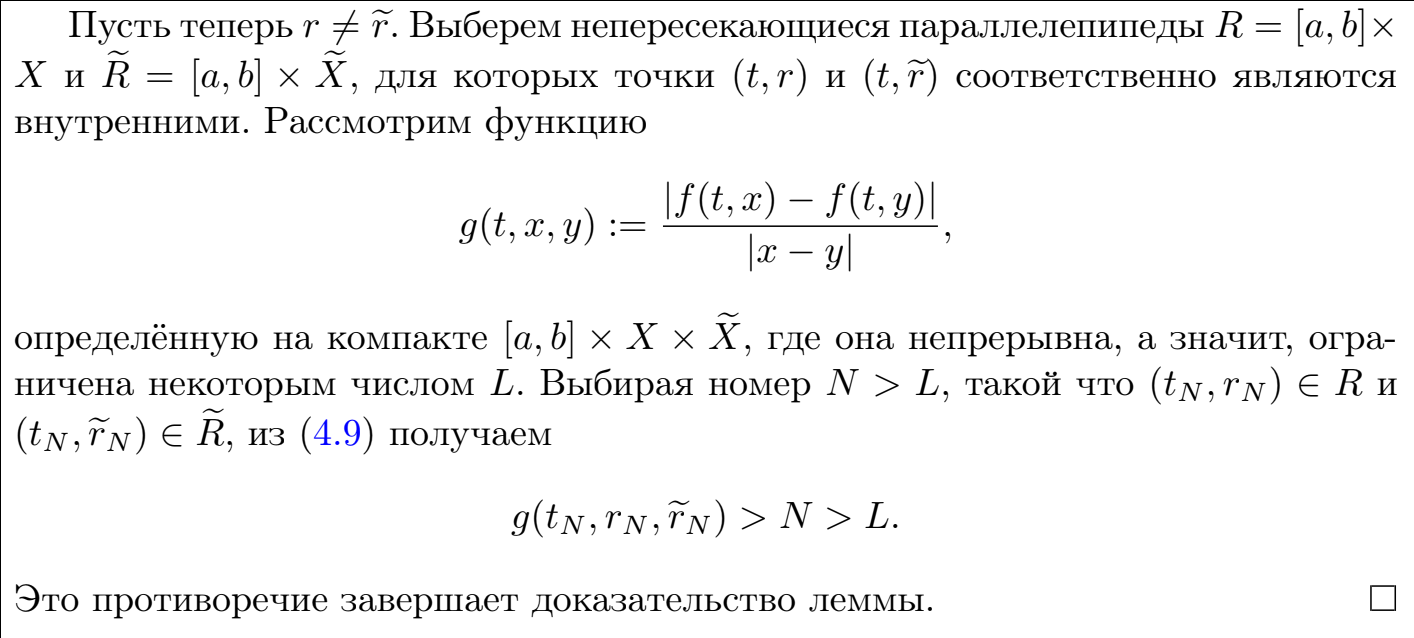
\includegraphics[scale=0.3]{images/7.png}
              %   \end{figure}
    \end{enumerate}
\end{proof}

\subsection*{8. Лемма Гронуолла. Теорема Пикара (доказательство единственности решения).}

\begin{lemma}[Гронуолл]
    \(\varphi\in C[a, b], t_0\in[a, b], \lambda,\mu \geq 0\) и
    \[\forall t\in[a, b] \ \ 0 \leq \varphi(t) \leq \lambda + \mu\left|\int_{t_0}^t \varphi(\tau)d\tau\right|\]
    Тогда
    \[\forall t\in[a, b] \ \ \varphi(t) \leq \lambda e^{\mu|t - t_0|}\]
\end{lemma}
\begin{proof}
    Рассмотрим \(t \geq t_0\) без потери общности.

    Рассмотрим случай \(\lambda > 0\) и пусть \(v(t) = \lambda + \mu\int_{t_0}^t \varphi(\tau)d\tau\). Тогда \(v'(t) = \mu\varphi(t) \leq \mu v(t)\). Таким образом, \(\cfrac{v'(t)}{v(t)} \leq \mu\). Проинтегрировав по \([t_0, t]\), получаем \(v(t) \leq v(t_0)e^{\mu(t - t_0)}\). Таким образом, \(\varphi(t) \leq v(t) \leq v(t_0)e^{\mu(t - t_0)} = \lambda e^{\mu(t - t_0)}\)

    Рассмотрим \(\lambda = 0\), тогда для любого \(\lambda_1\) верно \(\varphi(t) \leq \mu\int_{t_0}^t \varphi(\tau)d\tau < \lambda_1 + \mu\int_{t_0}^t \varphi(\tau)d\tau\), для этого уже доказали.

    При \(\lambda_1 \to 0\) получаем \(\varphi(t) \leq 0\).
\end{proof}

\begin{theorem}
    \(G\subset \R^{n + 1}_{t, r}\) --- область, \(f\in C(G \to \R^n)\cap \text{Lip}_{r, loc}(G), (t_0,r_0)\in G\). Тогда на отрезке Пеано существует решение задачи Коши \(\dot{r} = f(t, r), r(t_0) = r_0\) и оно единственно.
\end{theorem}

\begin{proof}
    Мы доказываем последний пункт, что решение \(\varphi\) единственно.

    Пусть \(\psi_1\) и \(\psi_2\) --- решения на \((a, b)\). По лемме об эквивалентном интегральном уравнении:
    \[\psi_1(t) = \int_0^t f(\tau, \psi_1(\tau))d\tau \quad \psi_2(t) = \int_0^t f(\tau, \psi_2(\tau))d\tau\]
    \[|\psi_1(t) - \psi_2(t)| \leq \int_0^t |f(\tau, \psi_1(\tau)) - f(\tau, \psi_2(\tau))|d\tau\]
    Пусть \([\alpha, \beta]\subset (a, b), a < 0, b > 0\).

    Т.к. графики \(\psi_1\) и \(\psi_2\) на \([\alpha, \beta]\) компактны, \(f(\tau, \psi_1(t))\) и то же самое для \(2\) Липшницевы, поэтому:
    \[|f(\tau, \psi_1(t)) - f(\tau, \psi_2(t))| \leq \tilde L|\psi_1(\tau) - \psi_2(\tau)|\]
    Итого:
    \[|\psi_1(t) - \psi_2(t)| \leq \tilde{L} \int_0^t |\psi_1(\tau) - \psi_2(\tau)|d\tau\]

    По лемме Гронуолла \(|\psi_1(t) - \psi_2(t)|\), т.к. \(\lambda = 0\), таким образом \(\psi_1\) и \(\psi_2\) совпадают на \([\alpha, \beta]\), а в силу произвольности они совпадают и на \((a, b)\)
\end{proof}

\subsection*{9. Теорема Пикара (доказательство существования решения).}

\begin{proof}
    Без потери общности \(t_0 = 0, r_0 = 0\). Рассмотрим правую часть отрезка Пеано \([0, h]\), для левой аналогично и решения можно сшить. Возьмём \(\Pi, M, h\) из определения отрезка Пеано.

    Рассмотрим последовательность функций:
    \begin{itemize}
        \item \(\varphi_0(t) = 0\)
        \item \(\varphi_{k + 1}(t) = \int_0^t f(\tau, \varphi_k(\tau))d\tau\)
    \end{itemize}

    У нас будет три этапа \textit{(в этом билете)}:
    \begin{enumerate}
        \item Докажем, что последовательность верно определена, т.е. \((t,\varphi_k(t))\in G\).
        \item Докажем, что последовательность равномерно сходится на \([0, h]\) к некоторой \(\varphi\)
        \item Докажем, что \(\varphi\) решает интегральное уравнение, эквивалентное искомому.
    \end{enumerate}

    \begin{enumerate}
        \item Докажем по индукции. База тривиальна. Переход:
              \[|\varphi_{k + 1}(t)| \leq \int_0^t |f(\tau, \varphi_k(\tau))|d\tau \leq Mt \leq Mh \leq \frac{Mb}{M} = b\]

        \item Докажем, что \(\forall \varepsilon > 0 \ \ \exists N : \forall t,m > N,k \ \ |\varphi_{m + k}(t) - \varphi_m(t)| \leq \varepsilon\)

              По лемме о достаточном условии Липшица \(f\in \text{Lip}_r(\Pi)\) с константой \(L\). Докажем по индукции, что
              \[|\varphi_{m + k}(t) - \varphi_m(t)| \leq \frac{ML^mt^{m + 1}}{(m + 1)!} \]
              , тогда искомое будет доказано, т.к. \(t < h\) и дробь \( \to 0\).

              База очевидна:
              \[|\varphi_{k}(t) - \varphi_0(t)| \leq \int_0^t |f(\tau, \varphi_{k - 1}(\tau))|d\tau \leq Mt\]

              Переход:
              \begin{align*}
                  |\varphi_{m + 1 + k}(t) - \varphi_{m + 1}(t)|
                   & \leq \int_0^t |f(\tau, \varphi_{m + k}(\tau)) - f(\tau, \varphi_m(\tau))|d\tau \\
                   & \leq \int_0^t L|(\tau, \varphi_{m + k}(\tau)) - (\tau, \varphi_m(\tau))|d\tau  \\
                   & \leq \int_0^t L\frac{ML^m\tau^{m + 1}}{(m + 1)!}d\tau                          \\
                   & \leq \frac{ML^{m + 1}t^{m + 2}}{(m + 2)!}d\tau                                 \\
              \end{align*}
        \item \[\varphi(t) = \lim_{m\to +\infty} \int_0^t f(\tau, \varphi_m(\tau)d\tau\]

              Т.к. \((t, \varphi_m(t))\in \Pi\), то и \((t, \varphi(t))\in \Pi\). Таким образом:
              \[|f(\tau, \varphi_m(\tau)) - f(\tau, \varphi(\tau))| \leq L|\varphi_m(\tau) - \varphi(\tau)|\]
              В силу равномерной сходимости \(\varphi_m\) мы получаем, что \(f(t, \varphi_m(t)) \to f(t, \varphi(t))\) при \(m \to +\infty\) равномерно. Тогда мы можем внести предел под знак интеграла по теореме о предельном переходе под знаком интеграла.
              \[\varphi(t) = \int_0^t f(\tau, \varphi(\tau)d\tau\]
              По лемме об эквивалентном интегральном уравнении получаем, что \(\varphi\) --- решение искомого уравнения.
    \end{enumerate}
\end{proof}

\subsection*{10. Теорема существования и единственности решения ЗК для уравнения $n$-го порядка. Следствие с более простыми условиями.}

\begin{theorem}
    \(G\subset \R^{n + 1}_{t, y, \dot{y}, \dots , y^{(n - 1)}}\) --- область, \(f\in C(G)\), \(f\in \text{Lip}_{(y, \dot{y}, \dots , y^{(n - 1)}), loc}(G), (t_0, y_0, \dot{y}_0, \dots , y^{(n-1)}_0)\in G\). Тогда в некоторой окрестности \(t_0\) есть решение задачи Коши для уравнения \(y^{(n)} = f(t, y, \dot{y}, \dots , y^{(n - 1)})\)
\end{theorem}

\begin{proof}
    Рассмотрим эквивалентную систему. Каждое из уравнений имеет единственное решение задачи Коши по теореме Пикара. По Пикару у эквивалентной системы есть решение.
\end{proof}

\begin{corollary}
    \(G\subset \R^{n + 1}_{t, y, \dot{y}, \dots , y^{(n - 1)}}\) --- область, \(f, f'_y, f'_{y'}, \dots , f'_{y^{(n - 1)}}\in C(G), (x_0, y_0, y_0', \dots , y_0^{(n - 1)})\in G\). Тогда в некоторой окрестности есть единственное решение задачи Коши для уравнения \(y^{(n)} = f(t, y, \dot{y}, \dots , y^{(n - 1)})\).
\end{corollary}

\begin{proof}
    Была лемма, по которой \(f\in \text{Lip}_{(y, \dot{y}, \dots , y^{(n - 1)}), loc}(G)\) и по теореме в этом билете.
\end{proof}

\subsection*{11. Критерий продолжимости.}

\begin{theorem}
    \(G\subset \R^{n + 1}_{t, r}\) --- область, \(f\in C(G \to \R^n)\). Тогда решение \(\varphi\) уравнения \(\dot{r} = f(t, r)\) на промежутке \([a, b)\) продолжимо вправо \(\Leftrightarrow\) \(\exists \lim\limits_{x \to b - 0} \varphi(x) = \tilde{r}\) и при этом \((b, \tilde{r})\in G\)
\end{theorem}

\begin{proof}\itemfix
    \begin{itemize}
        \item [\( \Rightarrow \)] Пусть \(\psi\) --- продолжение вправо \(\varphi\).

              Т.к. \(\psi\) непрерывна, то \(\varphi(b - 0) = \psi(b - 0) = \psi(b)\). Т.к. \(b\in \text{dom}\psi\), \((b, \psi(b))\in G\).

        \item [\( \Leftarrow \)] Доопределим \(\varphi\) на \([a, b]\). На \([a, b)\):

              \[\varphi(t) - \varphi(t_1) = \int_{t_1}^t \varphi'(\tau)d\tau = \int_{t_1}^t f(\tau, \varphi(\tau))d\tau\]

              Пусть \(t_1 \to b\).

              \[\varphi(t) = \tilde{r} + \int_b^t f(\tau, \varphi(\tau))d\tau\]

              По лемме об экв. интегральном уравнении \(\varphi\) --- решение задачи \(\dot{r} = f(t, r), r(b) = \tilde{r}\)

              По теореме Пеано есть решение \(\vartheta\) на \([b - h, b + h]\). Тогда можем сшить \(\vartheta, \varphi\) и получить \(\psi\), это будет решение \([a, b + h]\).
    \end{itemize}
\end{proof}

\subsection*{12. Теорема существования и единственности максимального решения.}

\begin{theorem}
    \(G\subset \R^{n + 1}_{t, r}\) --- область, \(f\in \text{Lip}_{r, loc}(G), f\in C(G \to \R^n), (t_0, r_0)\in G\)

    Тогда максимальное решение задачи Коши существует и единственно.
\end{theorem}
\begin{proof}
    Пусть все решения задачи Коши на интервалах образуют множество \(S\). По теореме Пеано \(|S| \neq 0\). Пусть для \(\varphi\in S\) область определения \((a_\varphi, b_\varphi)\). Пусть \((A,B) : = \bigcup\limits_{\varphi\in S}(a_\varphi, b_\varphi)\)

    Для \(t\in(a_\varphi, b_\varphi)\) пусть \(\psi(t) : = \varphi(t)\). Т.к. все решения задачи Коши совпадают \textit{(теорема Пикара)}, функция задана однозначно. Вполне очевидно, что \(\psi\) --- максимальное решение.

    Другого решения \(\vartheta\) нет, т.к. если \(\text{dom} \vartheta \neq \text{dom} \psi\), то одно из них не максимально, а иначе они равны.
\end{proof}

\subsection*{13. Теорема о выходе интегральной кривой за пределы любого компакта.}

\begin{theorem}
    Пусть $n \in \mathbb{N}$, $G \subset \mathbb{R}_{t,r}^{n+1}$ --- область, $f \in C(G \to \mathbb{R}^n)\cap Lip_{r,loc}(G)$, $\varphi$ --- максимальное решение на $(a,b)$ уравнения $\dot{r} = f(t,r)$, $K \subset G$ --- компакт. Тогда найдется $\Delta > 0$, такое что $(t, \varphi(t)) \notin K$ при всех $t \in (a, a + \Delta) \cup (b - \Delta, b)$.
\end{theorem}

\begin{proof}
    Заметим, что расстояние $\rho = \rho(K, \partial G)$ от компакта $K$ до границы $\partial G$ области $G$ положительно (иначе можно было бы построить последовательность точек из $K$, сходящейся к точке на границе, но $\partial G \cap K = \varnothing$). Если $\rho < +\infty$, положим $c = \frac{\rho}{2}$, иначе пусть $c = 1$.

    Вокруг каждой точки $(t', r') \in K$ построим содержащийся внутри $G$ параллелепипед
    \begin{equation*}
        \Pi(t',r') = \left\{(t,r) \in \mathbb{R}^{n+1}\, | \, |t-t'| \le c,\, |r - r'| \le c \right\}
    \end{equation*}
    и рассмотрим множество
    \begin{equation*}
        K_c = \bigcup_{(t',r') \in K} \Pi(t',r')
    \end{equation*}

    Поскольку $K$ --- компакт, то максимум нормы достигается, пусть это $d$. Если $(t,r)$ --- произвольная точка из $K_c$, то для некоторой точки $(t',r') \in K$ будет $(t,r) \in \Pi(t',r')$, поэтому
    \begin{equation*}
        |(t,r)| \le |(t,r) - (t',r')| + |(t',r')| \le c + d
    \end{equation*}
    Значит, множество $K_c$ ограничено.

    Докажем его замкнутость. Рассмотрим последовательность $\{(t_{m_k}, r_{m_k})\}$ точек из $K_c$, сходящуюся к $(t,r) \in \mathbb{R}^{n+1}$. Для каждой такой точки найдется параллелепипед $\Pi(t'_{m_k},r'_{m_k})$, которому она принадлежит. Раз $K$ --- компакт, то существует подпоследовательность $\{(t'_{m_k}, r'_{m_k})\}$, сходящаяся к некоторой точке $(t',r') \in K$. Переходя к пределу в неравенствах
    \begin{equation*}
        |t_{m_k} - t'_{m_k}| \le c, \quad |r_{m_k} - r'_{m_k}| \le c
    \end{equation*}
    находим $|t - t'| \le c$ и $|r - r'| \le c$. Следовательно $(t,r) \in K_c$.

    Таким образом, $K_c$ --- компакт, и функция $f$ достигает на нем максимального значения
    \begin{equation*}
        M = \max_{(t,r) \in K_c} |f(t,r)|
    \end{equation*}

    Теперь предположим, что утверждение теоремы неверно. Пусть $\Delta = \frac{h}{2}$, где $h = \min \{c, \frac{c}{M}\}$. Тогда при некотором $t_0 \in (b - \frac{h}{2}, b)$ будет $(t_0, \varphi(t_0)) \in K$.

    Рассмотрим ЗК $\dot{r} = f(t,r),\, r(t_0) = \varphi(t_0)$. По теореме Пеано она имеет решение $\psi$ на отрезке $[t_0 - h, t_0 + h]$. Пусть
    \begin{equation*}
        \widetilde{\varphi}(t) = \begin{cases}
            \varphi(t), \quad \text{если } t \in (a, t_0) \\
            \psi(t), \quad \text{если } t \in [t_0, t_0 + h]
        \end{cases}
    \end{equation*}

    По лемме о гладкой стыковке решений $\widetilde{\varphi}$ --- решение уравнения $\dot{r} = f(t,r)$ на $(a, t_0 + h)$. Функция $\widetilde{\varphi} \equiv \varphi$ на $(a,b) \cap (a, t_0 + h)$ по теореме Пикара. Но
    \begin{equation*}
        t_0 + h > b - \frac{h}{2} + h = b + \frac{h}{2} > b
    \end{equation*}
    то есть $\widetilde{\varphi}$ --- продолжение $\varphi$ вправо за точку $b$. Так как $\varphi$ по условию является максимальным решением, приходим к противоречию.
\end{proof}

\subsection*{14. Признак продолжимости решения системы, сравнимой с линейной. Теорема о существовании и единственности максимального решения ЛС.}

\begin{theorem}
    Пусть $G = (a,b) \times \mathbb{R}_r^n$, $f \in C(G \to \mathbb{R}^n) \cap Lip_{r,loc}(G)$, функции $u,v \in C(a,b)$ таковы, что для любых $(t,r) \in G$
    \begin{equation*}
        |f(t,r)| \le u(t)|r| + v(t)
    \end{equation*}
    Тогда каждое максимальное решение уравнения $\dot{r} = f(t,r)$ определено на $(a,b)$.
\end{theorem}

\begin{proof}
    По теореме о существовании и единственности максимального решения любая задача Коши с начальными данными $(t_0, r_0) \in G$ имеет единственное максимальное решение $\varphi$, заданное на некотором интервале $(\alpha, \beta)$. Докажем, что границы интервала $(\alpha, \beta)$ совпадают с границами интервала $(a,b)$. Пойдем от противного. Пусть, например, $\beta < b$. Принимая во внимание лемму о равносильном интегральном уравнении, при $t \in [t_0, \beta)$ находим
    \begin{equation*}
        \begin{aligned}
             & |\varphi(t)| = \left|r_0 + \int_{t_0}^t f(\tau, \varphi(\tau))d\tau \right| \le |r_0| + \int_{t_0}^t |f(\tau, \varphi(\tau))|d\tau \le \\
             & \le |r_0| + \int_{t_0}^t |u(\tau)||\varphi(\tau)|d\tau + \int_{t_0}^t |v(\tau)|d\tau
        \end{aligned}
    \end{equation*}

    Из непрерывности функций $u$ и $v$ вытекает их ограниченность на отрезке $[t_0, \beta]$. Следовательно, найдутся такие числа $\lambda, \mu \ge 0$, что при $t \in [t_0, \beta)$
    \begin{equation*}
        |\varphi(t)| \le \lambda + \mu \int_{t_0}^t |\varphi(s)|ds
    \end{equation*}
    Тогда по лемме Гронуолла
    \begin{equation*}
        |\varphi(t)| \le \lambda e^{\mu (t - t_0)} \le L
    \end{equation*}
    где $L = \lambda e^{\mu (\beta - t_0)}$. Отсюда следует, что график решения $\varphi$ не покидает компакт
    \begin{equation*}
        K = \left\{(t,r) \in G\, |\, t \in [t_0, \beta],\, |r| \le L \right\} \subset G
    \end{equation*}
    при $t \in [t_0, \beta)$, что противоречит теореме о выходе интегральной кривой за пределы компакта.
\end{proof}

\noindent \textbf{Определение.} \textbf{Линейной системой дифференциальных уравнений} называют систему вида
\begin{equation}
    \dot{r} = P(t)r + q(t) \label{lnsu}
\end{equation}
где $P \in M_n(C(a,b))$, $q \in C((a,b) \to \mathbb{R}^n)$.\\

\noindent \textbf{Теорема (существование и единственность максимального решения ЛС).} Пусть $P \in M_n(C(a,b))$, $q \in C((a,b) \to \mathbb{R}^n)$, $t_0 \in (a,b)$, $r_0 \in \mathbb{R}^n$. Тогда максимальное решение задачи Коши
\begin{equation}
    \begin{cases}
        \dot{r} = P(t)r + q(t) \\
        r(t_0) = r_0
    \end{cases} \label{zkls}
\end{equation}
существует, единственно и определено на интервале $(a,b)$.\\

\noindent \textbf{Доказательство.} Заметим, что правая часть системы $f(t,r) = P(t)r + q(t)$ и ее производная $f'_r = P(t)$ непрерывны в области $(a,b) \times \mathbb{R}^n$. Тогда существует единственное максимальное решение задачи \eqref{zkls} по теореме о \(!\exists\) максимального решения.

Имеем
\begin{equation*}
    |f(t,r)| \le |P(t)r| + |q(t)| \le n|P(t)||r| + |q(t)|
\end{equation*}
Так как функции $u(t) = n|P(t)|$ и $v(t) = |q(t)|$ непрерывны на $(a,b)$, то по признаку продолжимости системы, сравнимой с линейной, решение задачи \eqref{zkls} продолжимо на интервал $(a,b)$.

\subsection*{15. Формула Остроградского–Лиувилля для решений ЛОС.}

\textbf{Определение.} Если $q \equiv 0$ на $(a,b)$, то система \eqref{lnsu}, то есть
\begin{equation}
    \dot{r} = P(t)r \label{losu}
\end{equation}
называется \textbf{однородной}, в противном случае \textbf{неоднородной}.\\

\noindent \textbf{Определение.} \textbf{Определителем Вронского (вронскианом)} вектор-функций $\{r_k\}_{k=1}^n$, где $r_k=(x_{k1}, x_{k2}, \ldots, x_{kn})^T$, называют определитель
\begin{equation*}
    W(t) = det(r_1(t),r_2(t),\ldots, r_n(t)) = \begin{vmatrix}
        x_{11}(t) & x_{21}(t) & \ldots & x_{n1}(t) \\
        x_{12}(t) & x_{22}(t) & \ldots & x_{n2}(t) \\
        \ldots                                     \\
        x_{1n}(t) & x_{2n}(t) & \ldots & x_{nn}(t)
    \end{vmatrix}
\end{equation*}
\\
\noindent \textbf{Теорема (формула Остроградского-Лиувилля для решений ЛОС).} Пусть $t, t_0 \in (a,b)$, $P \in M_n(C(a,b))$, $r_1, r_2, \ldots, r_n$ --- решения системы \eqref{losu}. Тогда их вронскиан
\begin{equation*}
    W(t) = W(t_0)\exp \int_{t_0}^t \tr P(\tau)d\tau
\end{equation*}
\textbf{Доказательство.} Пусть $X$ --- матрица со столбцами $r_1, r_2, \ldots, r_n$, а $R_k$ --- ее $k$-ая строка. Используя формулу полного разложения определителя, нетрудно убедиться, что
\begin{equation*}
    \dot{W} = \det\begin{pmatrix}
        \dot{R}_1 \\
        R_2       \\
        \ldots    \\
        R_n
    \end{pmatrix} + \det\begin{pmatrix}
        R_1       \\
        \dot{R}_2 \\
        \ldots    \\
        R_n
    \end{pmatrix} + \ldots + \det\begin{pmatrix}
        R_1    \\
        R_2    \\
        \ldots \\
        \dot{R}_n
    \end{pmatrix}
\end{equation*}

Так как
\begin{equation*}
    \dot{X} = (\dot{r}_1, \dot{r}_2, \ldots, \dot{r}_n) = (Pr_1, Pr_2, \ldots, Pr_n) = PX
\end{equation*}
то $k$-ая строка матрицы $\dot{X}$ совпадает с $k$-ой строкой матрицы $PX$, то есть
\begin{equation*}
    \dot{R}_k = \sum_{k=1}^n p_{kj}R_j
\end{equation*}
где $p_{kj}$ --- элемент матрицы $P$ в $k$-ой строке и $j$-ом столбце.

Подставляя выражение для $\dot{R}_k$ в формулу для $\dot{W}$ и используя свойства определителя, находим
\begin{equation*}
    \dot{W} = p_{11}\det\begin{pmatrix}
        R_1    \\
        R_2    \\
        \ldots \\
        R_n
    \end{pmatrix} + p_{22}\det\begin{pmatrix}
        R_1    \\
        R_2    \\
        \ldots \\
        R_n
    \end{pmatrix} + \ldots + p_{nn}\det\begin{pmatrix}
        R_1    \\
        R_2    \\
        \ldots \\
        R_n
    \end{pmatrix} = W\,\tr P
\end{equation*}
Интегрируя полученное уравнение, приходим к требуемой формуле.

\subsection*{16. Общее решение ЛОС. Лемма о множестве фундаментальных матриц. Лемма об овеществлении.}

\textbf{Теорема (Общее решение ЛОС).} Пусть $P \in M_n(C(a,b))$. Тогда множество решений системы $\dot{r} = P(t)r$ образуют $n$-мерное линейное пространство.

\begin{proof}
    Пусть $t_0 \in (a,b)$, $\{a_k\}_{k=1}^n$ --- базис в $\mathbb{R}^n$. Тогда для любого $k \in [1 : n]$ существует $r_k$ --- решение задачи Коши $\dot{r} = P(t)r,\, r(t_0) = a_k$. Вронскиан этих решений $W(t_0) = \det(a_1, a_2, \ldots, a_n) \neq 0$. Тогда функции $\{r_k\}_{k=1}^n$ линейно независимы.

    Рассмотрим произвольное решение $r$ системы $\dot{r} = P(t)r$. Пусть $\{c_k\}_{k=1}^n$ --- координаты вектора $r(t_0)$ в базисе $\{a_k\}_{k=1}^n$. Положим
    \begin{equation*}
        \varphi = c_1r_1 + c_2r_2 + \ldots + c_nr_n
    \end{equation*}
    Ясно, что $\varphi$ --- решение системы $\dot{r} = P(t)r$, при этом $\varphi(t_0) = r_0$. Тогда $r \equiv \varphi$ в силу теоремы о единственности максимального решения ЛС.

    Таким образом, функции $\{r_k\}_{k=1}^n$ линейно независимы, и любое решение есть их линейная комбинация. Значит, $\{r_k\}_{k=1}^n$ --- базис в пространстве решений.
\end{proof}

\noindent \textbf{Определение.} \textbf{Фундаментальной системой решений} системы уравнений $\dot{r} = P(t)r$ называется совокупность ее $n$ линейно независимых решений.

\noindent \textbf{Определение.} \textbf{Фундаментальная матрица системы} $\dot{r} = P(t)r$ --- матрица, столбцы которой образуют фундаментальную систему решений.

\noindent \textbf{Лемма (о множестве фундаментальных матриц).} Пусть $\Phi$ --- фундаментальная матрица системы $\dot{r} = P(t)r$. Тогда $\left\{\Phi A \, | \, A \in M_n(\mathbb{R}), \, \det A \neq 0 \right\}$ --- множество всех фундаментальных матриц этой системы.

\begin{proof}
    Пусть $\Psi$ --- фундаментальная матрица системы $\dot{r} = P(t)r$. Тогда каждый ее столбец, будучи решением этой системы, является линейной комбинацией столбцов матрицы $\Phi$. Записывая коэффициенты разложения в столбцы матрицы $A$, имеем $\Psi = \Phi A$. А так как $det \Psi \neq 0$ и $\det \Phi \neq 0$, то и $\det A \neq 0$.

    Обратно, пусть $A \in M_n(\mathbb{R})$ --- произвольная невырожденная матрица. Тогда матрица $\Phi A$ состоит из решений, а ее определитель не обращается в ноль. Следовательно, эти решения линейно независимы, поэтому $\Phi A$ --- фундаментальная матрица.
\end{proof}

\noindent \textbf{Лемма (Об овеществлении).} Пусть $n \in \mathbb{N}$, $\Phi = (r_1,r_2,r_3,\ldots,r_n)$ --- фундаментальная матрица системы $\dot{r} = P(t)r$, при этом $r_1 = \overline{r}_2$. Тогда
\begin{equation*}
    \Psi = (\Re r_1, \Im r_1, r_3, \ldots, r_n)
\end{equation*}
--- фундаментальная матрица той же системы.

\begin{proof}
    Так как
    \begin{equation*}
        \begin{aligned}
             & \Re\, r_1 = \frac{1}{2}(r_1 + \overline{r}_1) = \frac{1}{2}r_1 + \frac{1}{2}r_2   \\
             & \Im\,r_1 = \frac{1}{2i}(r_1 - \overline{r}_1) = \frac{1}{2i}r_1 - \frac{1}{2i}r_2
        \end{aligned}
    \end{equation*}
    то
    \begin{equation*}
        \Psi = \Phi \begin{pmatrix}
            \begin{matrix}
                \frac{1}{2} & \frac{1}{2i}  \\
                \frac{1}{2} & -\frac{1}{2i}
            \end{matrix} & 0       \\
            0                          & E_{n-2}
        \end{pmatrix}
    \end{equation*}
    где $E_{n-2}$ --- единичная матрица порядка $n - 2$. По лемме о множестве фундаментальных матриц матрица $\Psi$ является фундаментальной.
\end{proof}

\subsection*{17. Теорема о фундаментальной системе решений ЛОС с постоянными коэффициентами (случай жорданова базиса общего вида). Определение и свойства матричной экспоненты (без доказательств). Решение задачи Коши при помощи матричной экспоненты.}

\textbf{Определение.} \textbf{Линейной системой дифференциальных уравнений с постоянными коэффициентами} называют линейную систему вида
\begin{equation}
    \dot{r} = Ar = q(t) \label{linpost}
\end{equation}
где $A \in M_n(\mathbb{C})$, $q \in C((a,b) \to \mathbb{C}^n)$.\\

\noindent \textbf{Лемма.} Пусть $n, k \in \mathbb{N}$, $A \in M_n(\mathbb{C})$, $h_1, h_2, \ldots, h_k$ --- жорданова цепочка, соответствующая $\lambda \in spec\, A$. Тогда функции
\begin{equation*}
    \begin{aligned}
         & \varphi_1(t) = e^{\lambda t}h_1                                                                         \\
         & \varphi_2(t) = e^{\lambda t}\left(\frac{t}{1!}h_1 + h_2\right)                                          \\
         & \ldots                                                                                                  \\
         & \varphi_k(t) = e^{\lambda t}\left(\frac{t^{k-1}}{(k-1)!}h_1 + \ldots + \frac{t}{1!}h_{k-1} + h_k\right)
    \end{aligned}
\end{equation*}
являются решениями системы $\dot{r} = Ar$.\\

\noindent \textbf{Доказательство.} Принимая во внимание определение жордановой цепочки, при $j \in [1 : k]$ имеем
\begin{equation*}
    \begin{aligned}
         & A\varphi_j = e^{\lambda t}\sum_{m=1}^j \frac{t^{j-m}}{(j-m)!}Ah_m = e^{\lambda t} \left(\frac{t^{j-1}}{(j-1)!}\lambda h_1 + \sum_{m=2}^j \frac{t^{j-m}}{(j-m)!}(\lambda h_m + h_{m - 1}) \right) = \\
         & = e^{\lambda t}\left(\lambda \sum_{m=1}^j \frac{t^{j - m}}{(j - m)!}h_m + \sum_{m = 2}^j \frac{t^{j-m}}{(j - m)!}h_{m-1} \right)
    \end{aligned}
\end{equation*}

Это же выражение получается при дифференцировании вектор-функции $\varphi_j$. Значит, $\dot{\varphi}_j = A\varphi_j$, что и требовалось доказать.\\

\noindent \textbf{Теорема (Случай жорданова базиса общего вида).} Пусть $A \in M_n(\mathbb{C})$, базис пространства $\mathbb{C}^n$ состоит из жордановых цепочек
\begin{equation*}
    \begin{aligned}
         & \lambda_1 \sim h_1, h_2, \ldots, h_k \\
         & \ldots                               \\
         & \lambda_d \sim u_1, u_2, \ldots, u_m
    \end{aligned}
\end{equation*}
соответствующих $\lambda_1, \ldots, \lambda_d \in spec\, A$. Тогда вектор-функции
\begin{equation*}
    \begin{aligned}
         & \varphi_1(t) = e^{\lambda_1 t}h_1, \quad \ldots, \quad \varphi_k(t) = e^{\lambda_1 t}\left(\frac{t^{k-1}}{(k-1)!}h_1 + \ldots + \frac{t}{1!}h_{k-1} + h_k \right) \\
         & \ldots                                                                                                                                                            \\
         & \psi_1(t) = e^{\lambda_d t}u_1, \quad \ldots, \quad \psi_m(t) = e^{\lambda_d t}\left(\frac{t^{m-1}}{(m-1)!}u_1 + \ldots + \frac{t}{1!}u_{m-1} + u_m \right)
    \end{aligned}
\end{equation*}
образуют фундаментальную систему решений системы $\dot{r} = Ar$.\\

\noindent \textbf{Доказательство.} По вышедоказанной лемме каждая из вектор-функций
\begin{equation*}
    \varphi_1, \ldots, \varphi_k, \ldots, \psi_1, \ldots, \psi_m
\end{equation*}
является решением. Их вронскиан
\begin{equation*}
    W(0) = det(h_1, \ldots, h_k, \ldots, u_1, \ldots, u_m) \neq 0
\end{equation*}
Тогда вектор-функции $\{\varphi_1, \ldots, \varphi_k, \ldots, \psi_1, \ldots, \psi_m\}$ линейно независимы, а значит, образуют фундаментальную систему решений.\\

\noindent \textbf{Определение.} \textbf{Матричной экспонентой} называется сумма ряда
\begin{equation*}
    e^{A} = \sum_{k = 0}^{\infty} \frac{A^k}{k!}
\end{equation*}
\\
\noindent \textbf{Свойства матричной экспоненты.} Пусть $A$, $B$, $J$, $T \in M_n(\mathbb{C})$, $det\, T \neq 0$, $t \in \mathbb{R}$. Тогда
\begin{enumerate}
    \item ряд, определяющий $e^A$, сходится
    \item если $AB = BA$, то $e^{A+B} = e^{A}e^{B}$
    \item $\frac{d}{dt}e^{At} = Ae^{At}$
    \item если $A = TJT^{-1}$, то $e^A = Te^JT^{-1}$
    \item если $A = diag(A_1, A_2, \ldots, A_d)$, то $e^A = diag(e^{A_1}, e^{A_2}, \ldots, e^{A_d})$
    \item если $J_s(\lambda)$ --- жорданова клетка размера $s$:
          \begin{equation*}
              J_s(\lambda) = \begin{pmatrix}
                  \lambda & 1       & 0       & \ldots & 0       \\
                  0       & \lambda & 1       & \ldots & 0       \\
                  0       & 0       & \lambda & \ldots & 0       \\
                  \ldots                                         \\
                  0       & 0       & 0       & \ldots & \lambda
              \end{pmatrix}
          \end{equation*}
          то
          \begin{equation*}
              e^{J_s(\lambda)t} = \begin{pmatrix}
                  1 & t & \frac{t^2}{2!} & \ldots & \frac{t^{s-1}}{(s-1)!} \\
                  0 & 1 & t              & \ldots & \frac{t^{s-2}}{(s-2)!} \\
                  0 & 0 & 1              & \ldots & \frac{t^{s-3}}{(s-3)!} \\
                  \ldots                                                   \\
                  0 & 0 & 0              & \ldots & 1
              \end{pmatrix}
          \end{equation*}
\end{enumerate}

\noindent \textbf{Теорема.} Пусть $A \in M_n(\mathbb{C})$. Тогда матрица $e^{At}$ является фундаментальной матрицей системы $\dot{r} = Ar$.

\noindent \textbf{Доказательство.} По свойствам матричной экспоненты будет $\frac{d}{dt}e^{At} = Ae^{At}$. Следовательно, каждый столбец матрицы $e^{At}$ --- решение системы $\dot{r} = Ar$. Соответствующий вронскиан
\begin{equation*}
    W(0) = \det\, e^{A\cdot 0} = \det E_n = 1
\end{equation*}
где $E_n$ --- единичная матрица порядка $n$. Отсюда следует, что $e^{At}$ --- фундаментальная матрица.\\

\noindent \textbf{Следствие.} Пусть $A \in M_n(\mathbb{C})$, $t_0 \in \mathbb{R}$, $r_0 \in \mathbb{C}^n$. Тогда решением задачи
\begin{equation*}
    \dot{r} = Ar, \quad r(t_0) = r_0
\end{equation*}
является вектор-функция $\varphi(t) = e^{A(t - t_0)}r_0$

\subsection*{18. Общее решение ЛНС и метод вариации постоянных.}

\textbf{Теорема (Общее решение ЛНС).} Пусть $P \in M_n(C(a,b))$, $q \in C((a,b) \to \mathbb{R}^n)$, $\varphi$ --- решение системы
\begin{equation}
    \dot{r} = P(t)r + q(t) \label{lnusyst2}
\end{equation}
$\Phi$ --- фундаментальная матрица системы
\begin{equation*}
    \dot{r} = P(t)r
\end{equation*}
Тогда общее решение неоднородной системы \eqref{lnusyst2} имеет вид
\begin{equation*}
    r = \Phi C + \varphi, \quad C \in \mathbb{R}^n
\end{equation*}
\textbf{Доказательство.} Пусть $r$ --- произвольное решение \eqref{lnusyst2}. Тогда
\begin{equation*}
    \dot{r} = Pr + q
\end{equation*}
Функция $\varphi$ удовлетворяет такому же соотношению:
\begin{equation*}
    \dot{\varphi} = P\varphi + q
\end{equation*}
Вычитая эти равенства, находим
\begin{equation*}
    (r - \varphi)' = P(r - \varphi)
\end{equation*}
Значит, найдется вектор-столбец $C \in \mathbb{R}^n$, такой что
\begin{equation*}
    r - \varphi = \Phi C
\end{equation*}

Верно и обратное: любая функция вида $\Phi C + \varphi$ являются решением \eqref{lnusyst2}, что проверяется непосредственной подстановкой.\\

\noindent \textbf{Теорема (метод вариации постоянных для ЛНС).} Пусть $\Phi$ --- фундаментальная матрица системы $\dot{r} = P(t)r$, $P \in M_n(C(a,b))$, $q \in C((a,b) \to \mathbb{R}^n)$. Тогда если вектор-функция $C$ пробегает все решения системы
\begin{equation*}
    \Phi\dot{C} = q
\end{equation*}
то $r = \Phi C$ пробегает все решения системы \eqref{lnusyst2}\\

\noindent \textbf{Доказательство.} Опираясь на формулу для обратной матрицы, использующей алгебраические дополнения, заключаем, что $\Phi^{-1} \in M_n(C(a,b))$. Поэтому
\begin{equation*}
    C(t) = \int \Phi^{-1}q + A
\end{equation*}
где $A$ --- вектор произвольных постоянных. Тогда требуется доказать, что общее решение системы \eqref{lnusyst2} имеет вид
\begin{equation*}
    r = \Phi A + \Phi \int \Phi^{-1}q
\end{equation*}
По теореме об общем решении ЛНС достаточно показать, что второе слагаемое в правой части --- частное решение системы \eqref{lnusyst2}. Убедимся в этом подстановкой:
\begin{equation*}
    \dot{\Phi}\int \Phi^{-1}q + \Phi\Phi^{-1}q = P(t)\Phi \int \Phi^{-1}q + q
\end{equation*}
Это верное тождество, поскольку $P(t)\Phi = \dot{\Phi}$.

\subsection*{19. Теорема об изоморфизме решений ЛОС и ЛОУ, формула Остроградского–Лиувилля для решений ЛОУ. Метод вариации постоянных для ЛНУ.}

\textbf{Определение.} \textbf{Линейным дифференциальным уравнением} порядка $n$ называется уравнение вида
\begin{equation}
    y^{(n)} + p_{n-1}(t)y^{(n - 1)} + \ldots + p_1(t)\dot{y} + p_0(t)y = q(t) \label{lndu}
\end{equation}
где $p_0, p_1, \ldots, p_{n-1}, q \in C(a,b)$.\\

\noindent \textbf{Определение.} Если $q \equiv 0$ на $(a,b)$, то уравнение \eqref{lndu}, то есть
\begin{equation}
    y^{(n)} + p_{n-1}(t)y^{(n - 1)} + \ldots + p_1(t)\dot{y} + p_0(t)y = 0 \label{lnou}
\end{equation}
называется \textbf{однородным}, в противном случае --- \textbf{неоднородным}.\\

\noindent \textbf{Лемма (О равносильной ЛС).} Если функция $y$ --- решение уравнения \eqref{lndu} на $(a,b)$, то вектор-функция $\Lambda_n y = (y, \dot{y}, \ldots, y^{(n-1)})$ --- решение системы
\begin{equation}
    \dot{r} = P(t)r + Q(t) \label{ravn}
\end{equation}
где
\begin{equation*}
    P = \begin{pmatrix}
        0    & 1    & 0    & \ldots & 0          \\
        0    & 0    & 1    & \ldots & 0          \\
        \ldots                                   \\
        0    & 0    & 0    & \ldots & 1          \\
        -p_0 & -p_1 & -p_2 & \ldots & -p_{n - 1}
    \end{pmatrix}, \quad Q = \begin{pmatrix}
        0      \\
        0      \\
        \ldots \\
        0      \\
        q
    \end{pmatrix}
\end{equation*}

И наоборот, если $r = (y_1, y_2, \ldots, y_n)$ --- решение системы \eqref{ravn}, то $y_1$ --- решение \eqref{lndu} на $(a,b)$ и $r = \Lambda_n y_1$.\\

\noindent \textbf{Теорема (Об изоморфизме).} Пусть $p_0, p_1, \ldots, p_{n-1} \in C(a,b)$. Тогда множество решений однородного уравнения \eqref{lnou} является линейным пространством, изоморфным пространству решений системы
\begin{equation}
    \dot{y} = P(t)y \label{izomorf}
\end{equation}
где матрица $P$ та же, что и в лемме о равносильной ЛС. При этом изоморфизм устанавливается отображением $\Lambda_n$.\\

\noindent \textbf{Доказательство.} Любое решение уравнения \eqref{lnou} по теореме о существовании и единственности максимального решения ЛУ является элементом линейного пространства $C^n(a,b)$. Кроме того, сумма двух решений, а также решение, умноженное на произвольное число, также являются решениями. Поэтому множество всех решений само образует линейное пространство.

Лемма о равносильной ЛС устанавливает биекцию между решениями уравнения и равносильной системы. Отображение $\Lambda_n$ линейно. Таким образом, $\Lambda_n$ --- изоморфизм.\\

\noindent \textbf{Определение.} \textbf{Определителем Вронского} (или \textbf{вронскианом}) функций $y_1, y_2, \ldots, y_n \in C^{n-1}(a,b)$ называют
\begin{equation*}
    W(t) = \begin{vmatrix}
        y_1(t)         & y_2(t)         & \ldots & y_n(t)         \\
        \dot{y}_1(t)   & \dot{y}_2(t)   & \ldots & \dot{y}_n(t)   \\
        \ldots                                                    \\
        y_1^{(n-1)}(t) & y_2^{(n-1)}(t) & \ldots & y_n^{(n-1)}(t)
    \end{vmatrix}
\end{equation*}

\noindent \textbf{Теорема (Формула Остроградского-Лиувилля для решений ЛОУ).} Пусть $t, t_0 \in (a,b)$, $p_0, p_1, \ldots, p_{n-1} \in C(a,b)$, $\{y_k\}_{k=1}^n$ --- решения линейного однородного уравнения \eqref{lnou}. Тогда вронскиан этих решений
\begin{equation*}
    W(t) = W(t_0)\exp \int_{t_0}^t (-p_{n-1}(\tau))d\tau
\end{equation*}
\textbf{Доказательство.} Принимая во внимание формулу Остроградского-Лиувилля для решений ЛОС и лемму о равносильной ЛС, находим
\begin{equation*}
    \begin{aligned}
         & W(y_1,\ldots, y_n) = W(\Lambda y_1,\ldots, \Lambda y_n) =                                  \\
         & = W(t_0)\exp \int_{t_0}^t tr\,P(\tau)d\tau = W(t_0)\exp \int_{t_0}^t (-p_{n-1}(\tau))d\tau
    \end{aligned}
\end{equation*}

\noindent \textbf{Теорема (метод вариации постоянных для ЛНУ).} Пусть $\{y_k\}_{k=1}^n$ --- фундаментальная система решений однородного уравнения \eqref{lnou}. Тогда если функции $\{C_k\}$ пробегают все решения системы
\begin{equation*}
    \begin{pmatrix}
        y_1         & y_2         & \ldots & y_n          \\
        \dot{y}_1   & \dot{y}_2   & \ldots & \dot{y}_n    \\
        \ldots                                            \\
        y_1^{(n-2)} & y_2^{(n-2)} & \ldots & y_n^{(n -2)} \\
        y_1^{(n-1)} & y_2^{(n-1)} & \ldots & y_n^{(n-1)}
    \end{pmatrix}
    \begin{pmatrix}
        \dot{C}_{1}   \\
        \dot{C}_{2}   \\
        \ldots        \\
        \dot{C}_{n-1} \\
        \dot{C}_{n}
    \end{pmatrix}
    =
    \begin{pmatrix}
        0      \\
        0      \\
        \ldots \\
        0      \\
        q
    \end{pmatrix}
\end{equation*}
то $y = \displaystyle\sum_{k = 1}^n C_ky_k$ пробегает все решения уравнения \eqref{lndu}.\\

\noindent \textbf{Доказательство.} По теореме о методе вариации постоянных для ЛС общее решение системы, равносильной уравнению \eqref{lndu}, имеет вид
\begin{equation*}
    r = \sum_{k=1}^n C_k \Lambda y_k
\end{equation*}
где функции $C_1, \ldots, C_n$ удовлетворяют системе
\begin{equation*}
    (\Lambda y_1, \ldots, \Lambda y_n)
    \begin{pmatrix}
        \dot{C}_{1}   \\
        \ldots        \\
        \dot{C}_{n-1} \\
        \dot{C}_{n}
    \end{pmatrix}
    =
    \begin{pmatrix}
        0      \\
        \ldots \\
        0      \\
        q
    \end{pmatrix}
\end{equation*}

По лемме о равносильной ЛС первая строка вектора $r$ --- общее решение уравнения \eqref{lndu}.

\subsection*{20. Общее решение ЛОУ с постоянными коэффициентами.}

\textbf{Определение.} \textbf{Линейным дифференциальным уравнением с постоянными коэффициентами} называют уравнение вида
\begin{equation}
    y^{(n)} + a_{n - 1}y^{(n-1)} + \ldots + a_1\dot{y} + a_0y = f(t) \label{lupost}
\end{equation}
где $a_0, a_1, \ldots, a_{n-1} \in \mathbb{C}$, $f \in C(a,b)$.\\

В дальнейшем для краткости используется обозначение
\begin{equation*}
    Ly = \frac{d^n}{dt^n}y + a_{n-1}\frac{d^{n-1}}{dt^{n-1}}y + \ldots + a_1\frac{d}{dt}y + a_0y = \left(\sum_{k = 0}^n a_k\frac{d^k}{dt^k} \right)y
\end{equation*}
где $a_n = 1$. При помощи оператора $L$ уравнение \eqref{lupost} записывается в виде
\begin{equation*}
    Ly = f(t)
\end{equation*}

Рассмотрим линейное однородное уравнение
\begin{equation}
    Ly = 0 \label{lodnpost}
\end{equation}
Применяя оператор $L$ к функции $e^{\lambda t}$, находим
\begin{equation*}
    L(e^{\lambda t}) = \sum_{k = 0}^n a_k\frac{d^k}{dt^k}e^{\lambda t} = \left(\sum_{k = 0}^n a_k\lambda^k \right)e^{\lambda t}
\end{equation*}

\noindent \textbf{Определение.} Многочлен
\begin{equation*}
    p(\lambda) = \lambda^n + a_{n-1}\lambda^{n-1} + \ldots + a_1\lambda + a_0
\end{equation*}
называется \textbf{характеристическим многочленом} уравнения \eqref{lupost}, а его корни --- \textbf{характеристическими числами} уравнения \eqref{lupost}.\\

Если $\lambda$ --- корень характеристического многочлена, то получаем $L(e^{\lambda t}) \equiv 0$. Верно и обратное: если $e^{\lambda t}$ --- решение однородного уравнения \eqref{lodnpost}, то $\lambda$ --- корень многочлена $p$. Докажем более общее утверждение.\\

\noindent \textbf{Лемма.} Пусть $\lambda \in \mathbb{C}$ --- корни кратности $m \in \mathbb{N}$ характеристического многочлена уравнения \eqref{lodnpost}. Тогда функции
\begin{equation*}
    e^{\lambda t}, te^{\lambda t}, \ldots, t^{m-1}e^{\lambda t}
\end{equation*}
являются решениями \eqref{lodnpost}.\\

\noindent \textbf{Доказательство.} Убедимся подстановкой в уравнение \eqref{lodnpost}, что указанные функции являются решениями.

Пусть $k \in [0 : m-1]$. Считая $\lambda$ переменной, в силу бесконечной дифференцируемости функции $e^{\lambda t}$ при любом $j \in \mathbb{Z}_{+}$ будет
\begin{equation*}
    \frac{\partial^j}{\partial t^j}\frac{\partial^k}{\partial \lambda^k}e^{\lambda t} = \frac{\partial^k}{\partial\lambda^k}\frac{\partial^j}{\partial t^j}e^{\lambda t}
\end{equation*}
Тогда
\begin{equation*}
    L(t^ke^{\lambda t}) = L\left(\frac{\partial^k}{\partial\lambda^k}e^{\lambda t} \right) = \frac{\partial^k}{\partial\lambda^k}L(e^{\lambda t})
\end{equation*}
Применяя формулу Лейбница, имеем
\begin{equation*}
    \frac{\partial^k}{\partial\lambda^k}L(e^{\lambda t}) = \frac{\partial^k}{\partial\lambda^k} (p(\lambda)e^{\lambda t}) = \sum_{j = 0}^k C_k^j p^{(j)}(\lambda)\frac{\partial^{k - j}}{\partial\lambda^{k - j}} e^{\lambda t}
\end{equation*}
Подставляя вместо $\lambda$ корень кратности $m$ многочлена $p$, получаем ноль, поскольку при $j \in [0 : k]$ обнуляются значения $p^{(j)}(\lambda)$.\\

\noindent \textbf{Лемма (Линейная независимость квазиодночленов).} Пусть $k_j \in \mathbb{Z}_{+}$, $\lambda_j \in \mathbb{C}$ при $j \in [1 : n]$, $\{(k_j,\lambda_j)\}_{j=1}^n$ --- различные пары чисел. Тогда функции $\{t^{k_j}e^{\lambda_jt}\}_{j=1}^n$ линейно независимы на любом промежутке из $\mathbb{R}$.\\

\noindent \textbf{Доказательство.} Разобьем множество пар $(k_1, \lambda_1), \ldots, (k_n, \lambda_n)$ на группы с одинаковым вторым элементом. Если такая группа одна, то линейная независимость следует из линейной независимости одночленов.

Допустим, что линейная независимость доказана, если количество групп равно $m$. Предположим, что в случае $m + 1$ группы некоторая нетривиальная линейная комбинация этих функций тождественно равна нулю. Объединяя слагаемые с одинаковыми экспонентами и изменяя нумерацию чисел $\lambda_i$, имеем
\begin{equation*}
    p_1(t)e^{\lambda_1 t} + p_2(t)e^{\lambda_2 t} + \ldots + p_{m+1}(t)e^{\lambda_{m+1}t} \equiv 0
\end{equation*}
где $p_i$ --- многочлены, а числа $\lambda_i$ различны. Деля обе части на $e^{\lambda_{m+1}t}$, получаем
\begin{equation*}
    p_1(t)e^{(\lambda_1 - \lambda_{m+1}) t} + p_2(t)e^{(\lambda_2 - \lambda_{m+1}) t} + \ldots + p_m(t)e^{(\lambda_m - \lambda_{m+1}) t} + p_{m+1}(t) \equiv 0
\end{equation*}

Дифференцируя это тождество $deg\, p_{m+1} + 1$ раз, находим
\begin{equation}
    q_1(t)e^{(\lambda_1 - \lambda_{m+1}) t} + q_2(t)e^{(\lambda_2 - \lambda_{m+1}) t} + \ldots + q_m(t)e^{(\lambda_m - \lambda_{m+1}) t} \equiv 0 \label{diffeq}
\end{equation}
где при всех $i \in [1:m]$ многочлен $q_i$ имеет ту же степень, что и $p_i$.

Значит, если для некоторого $i$ будет $p_i \not\equiv 0$, то и $q_i \not\equiv 0$. Следовательно, в левой части тождества \eqref{diffeq} находится нетривиальная линейная комбинация квазиодночленов. Это противоречит индукционному предположению.\\

\noindent \textbf{Теорема (Общее решение ЛОУ с постоянными коэффициентами).} Пусть $\lambda_1, \lambda_2, \ldots, \lambda_s \in \mathbb{C}$ --- характеристические числа уравнения \eqref{lodnpost} кратностей $m_1, m_2, \ldots, m_s \in \mathbb{N}$. Тогда функции
\begin{equation}
    \begin{aligned}
         & e^{\lambda_1 t}, te^{\lambda_1 t}, \ldots, t^{m_1 - 1}e^{\lambda_1 t} \\
         & \ldots                                                                \\
         & e^{\lambda_s t}, te^{\lambda_s t}, \ldots, t^{m_s - 1}e^{\lambda_s t}
    \end{aligned} \label{fundsyst}
\end{equation}
образуют фундаментальную систему решений уравнения \eqref{lodnpost}.\\

\noindent \textbf{Доказательство.} Указанные функции являются решениями \eqref{lodnpost}, а по лемме о линейной независимости квазиодночленов они линейно независимы. Так как сумма всех кратностей равна порядку уравнения, то эти функции образуют фундаментальную систему решений.

\subsection*{21. Теорема об устойчивости ЛОС с постоянными коэффициентами.}
\textbf{Определение.} \textbf{Точкой покоя}, или \textbf{положением равновесия}, или \textbf{стационарным состоянием} системы $\dot{r} = f(r)$ называют точку $r_0$, такую что $f(r_0) = 0$.\\

\noindent \textbf{Определение.} Положение равновесия $r = 0$ автономной системы $\dot{r} = f(r)$ называется \textbf{усточивым (по Ляпунову)}, если для любой $\varepsilon$-окрестности нуля найдется такая $\delta$-окрестность нуля, что любое решение, выходящее из этой $\delta$-окрестности, во все будущие моменты времени отличается от нуля менее, чем на $\varepsilon$. То есть
\begin{equation*}
    \forall \varepsilon > 0 \, \exists \delta > 0:\, |r_0| < \delta \implies \forall t \ge 0 \, |r(t,0,r_0)| < \varepsilon
\end{equation*}
В противном случае положение равновесия называется \textbf{неустойчивым}.\\

\noindent \textbf{Определение.} Положение равновесия $r = 0$ автономной системы $\dot{r} = f(r)$ называется \textbf{асимптотически устойчивым}, если
\begin{itemize}
    \item $r = 0$ устойчиво
    \item все решения, начинающиеся в некоторой окрестности нуля, в будущем стремятся к нулю, то есть
          \begin{equation*}
              \exists \delta > 0:\, |r_0| < \delta \implies r(t,0,r_0) \to 0\, \text{при } t \to +\infty
          \end{equation*}
\end{itemize}

\noindent \textbf{Лемма} Пусть $\varphi$ --- решение системы $\dot{r} = f(t,r)$. Тогда $\varphi$ устойчиво (асимптотически устойчиво), если и только если устойчиво (асимптотически устойчиво) решение $s = 0$ системы
\begin{equation*}
    \dot{s} = f(t, s + \varphi) - f(t, \varphi)
\end{equation*}
\noindent \textbf{Доказательство.} Положим $s = r - \varphi$. Пусть $\dot{r} = f(t,r)$, тогда
\begin{equation*}
    \dot{s} = \dot{r} - \dot{\varphi} = f(t,r) - f(t,\varphi) = f(t, s + \varphi) - f(t,\varphi)
\end{equation*}
Получаем, что $s = 0$ --- решение системы $\dot{s} = f(t, s + \varphi) - f(t,\varphi)$. Остается сопоставить определение устойчивости (асимптотической устойчивости) для решения $\varphi$ исходной и решения $s = 0$ новой системы.\\

Из вышедоказанной леммы следует, что решение $\varphi$ линейной системы
\begin{equation*}
    \dot{r} = P(t)r + q(t)
\end{equation*}
устойчиво (асимптотически устойчиво), если и только если устойчиво (асимптотически устойчиво) решение $r = 0$ соответствующей линейной однородной системы
\begin{equation*}
    \dot{r} = P(t)r
\end{equation*}
Отсюда, в частности, вытекает, что все решения линейной системы имеют одинаковый характер устойчивости, поэтому можно говорить об устойчивости линейной системы.\\

\noindent \textbf{Теорема (Устойчивость ЛОС с постоянными коэффициентами).} Пусть $A \in M_n(\mathbb{R})$. Тогда система
\begin{equation}
    \dot{r} = Ar \label{lodnpost2}
\end{equation}
\begin{enumerate}
    \item асимптотически устойчива, если $Re \lambda < 0$ для всех $\lambda \in spec\, A$
    \item устойчива, если для каждого $\lambda \in spec\, A$ либо $Re\lambda < 0$, либо $Re \lambda = 0$ и алгебраическая кратность числа $\lambda$ совпадает с геометрической
    \item неустойчива, если найдется $\lambda \in spec\, A$, такое что либо $Re \lambda > 0$, либо $Re\lambda = 0$ и алгебраическая кратность числа $\lambda$ больше геометрической
\end{enumerate}
\noindent \textbf{Доказательство.} Через $T$ обозначим матрицу перехода к жорданову базису матрицы $A$, $J$ --- жорданова форма матрицы $A$.

Любое решение системы \eqref{lodnpost2} имеет вид
\begin{equation*}
    r(t) = e^{At}r(0) = Te^{Jt}T^{-1}r(0)
\end{equation*}
Принимая во внимание лемму о норме матрицы, получаем
\begin{equation}
    |r(t)| \le n^3 |T||e^{Jt}||T^{-1}||r(0)| = K |e^{Jt}||r(0)| \label{norm}
\end{equation}
где $K > 0$ не зависит от $t$. Обозначим через $a_{ij}(t)$ элементы матрицы $e^{Jt}$.
\begin{enumerate}
    \item Каждая функция $a_{ij}(t)$ имеет вид $Ce^{\lambda t}t^k$, где $\lambda$ --- одно из собственных чисел. Поскольку $Re \lambda < 0$, то для всех $i, j$ будет $a_{ij}(t) \to 0$ при $t \to +\infty$, следовательно,
          \begin{equation*}
              |e^{Jt}| \to 0 \quad \text{при } t \to +\infty
          \end{equation*}
          Тогда из оценки \eqref{norm} следует устойчивость и асимптотическая устойчивость нулевого решения.
    \item Каждая функция $a_{ij}(t)$ имеет вид $Ce^{\lambda t}t^k$, но теперь $k = 0$, если $Re \lambda = 0$. Следовательно, существует такое число $M$, что при всех $t \le 0$
          \begin{equation*}
              |e^{Jt}| < M
          \end{equation*}
          Поэтому из оценки \eqref{norm} следует устойчивость нулевого решения.
    \item Пусть существует собственное число $\lambda = \alpha + i\beta$, где $\alpha > 0$. Обозначим через $h$ соответствующий собственный вектор. Тогда вектор-функция
          \begin{equation*}
              \varphi(t) = e^{\lambda t}h
          \end{equation*}
          является комплексным решением \eqref{lodnpost2}.

          Если же имеется собственное число $\lambda = i\beta$, $\beta \neq 0$, алгебраическая кратность которого больше геометрической, то система \eqref{lodnpost2} имеет комплексное решение
          \begin{equation*}
              \varphi(t) = e^{i\beta t}(th_1 + h_2)
          \end{equation*}
          где $h_1, h_2$ --- собственный и присоединенный вектор, соответствующие число $\lambda$.

          Заметим, что в обоих случаях $|\varphi(t)| \to +\infty$ при $t \to +\infty$. Следовательно, хотя бы одна из вектор-функций, $Re\varphi(t)$ или $Im\varphi(t)$, является неограниченным вещественным решением \eqref{lodnpost2}. Пусть таковой является $Re\varphi(t)$. Тогда выбирая в качестве начального условия
          \begin{equation*}
              r(0) = \mu Re\varphi(0)
          \end{equation*}
          при достаточно малом $\mu$, получаем неограниченное решение с начальным значением в сколь угодно малой окрестности нуля. Отсюда следует, что нулевое решение неустойчиво.
\end{enumerate}

\subsection*{22. Классификация точек покоя ЛОС 2-го порядка (случай вещественных корней).}

Исследуем подробно поведение траекторий в окрестности точки покоя линейной системы
\begin{equation*}
    \dot{r} = Ar
\end{equation*}
если $A \in M_2(\mathbb{R})$. Пусть $\det A \neq 0$, тогда имеется единственное положение равновесия $r = 0$ и собственные числа $\lambda_1, \lambda_2$ матрицы $A$ отличны от нуля.\\

\noindent \textbf{Случай $\lambda_1 \neq \lambda_2$}

Перейдем в систему координат $u, v$, связанную с собственным базисом $h_1, h_2$. Подставляя в уравнение $r = Ts$, где $s = (u, v)^T$, $T = (h_1, h_2)$, получаем
\begin{equation*}
    T\dot{s} = ATs
\end{equation*}
Умножая слева на $T^{-1}$, находим
\begin{equation*}
    \dot{s} = T^{-1}ATs
\end{equation*}
Так как $T^{-1}AT = diag(\lambda_1, \lambda_2)$, то в новых координатах система имеет вид
\begin{equation*}
    \begin{cases}
        \dot{u} = \lambda_1 u \\
        \dot{v} = \lambda_2 v
    \end{cases}
\end{equation*}
Ее решение $u = C_1e^{\lambda_1 t}$, $v = C_2e^{\lambda_2 t}$.

Если одна, и только одна из констант $C_1$ и $C_2$ равна нулю, то получаем параметрическое задание одной из полуосей. Заметим еще, что изменение знака одной из констант преобразует фазовую траекторию в симметричную ей относительно координатной оси. Таким образом, достаточно изучить фазовый портрет только в первой четверти.

Пусть $C_1 > 0$, $C_2 > 0$. Выражая $t$ через $u$ и подставляя в выражение для $v$, находим
\begin{equation*}
    v = C_2\left(\frac{u}{C_1} \right)^{\frac{\lambda_2}{\lambda_1}} = Cu^{\frac{\lambda_2}{\lambda_1}}
\end{equation*}

При $0 < \lambda_1 < \lambda_2$ получается семейство парабол. Функции $u$ и $v$ возрастают, следовательно, фазовые траектории расходятся от начала координат. Отражая траектории относительно координатных осей, получаем фазовый портрет во всей плоскости (см. \hyperref[neustuzel]{рисунок}). Такая точка покоя называется \textbf{неустойчивый узел}.

\begin{figure}[H]\label{neustuzel}
    \center{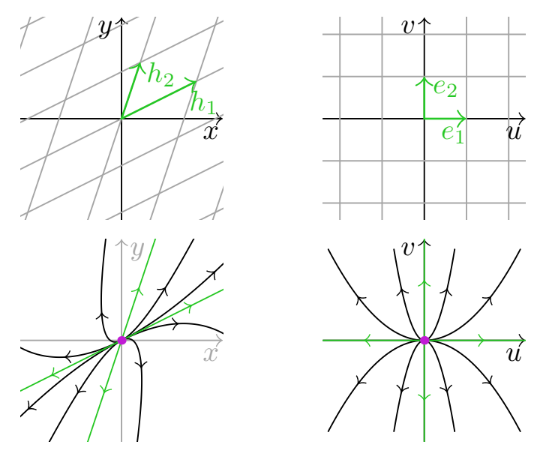
\includegraphics[scale=0.5]{images/neust_uzel.png}}
    \caption{Неустойчивый узел в старой и новой системе координат}
\end{figure}

При возвращении к прежней системе координат фазовый портрет исказится, но качественное поведение траекторий не изменится. Это замечание относится и ко всем последующим случаям.

Если $\lambda_2 < \lambda_1 < 0$, то уравнение фазовых траекторий не меняется, но изменяется направление движения. Теперь фазовые точки стремятся к началу координат. Соответствующее положение равновесия --- \textbf{устойчивый узел} (см. \hyperref[ustuzel]{рисунок}).

\begin{figure}[H]\label{ustuzel}
    \center{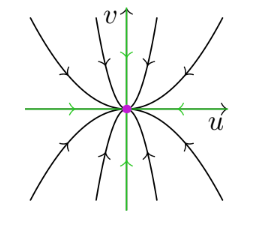
\includegraphics[scale=0.5]{images/ust_uzel.png}}
    \caption{Устойчивый узел}
\end{figure}

Если $\lambda_1 < 0 < \lambda_2$, то $v = Cu^{\frac{\lambda_2}{\lambda_1}}$ --- уравнение гиперболы. Соотношения $u = C_1e^{\lambda_1 t} \to 0$, $v = C_2e^{\lambda_2 t} \to \infty$ при $t \to +\infty$ дают представление о направлении движения вдоль фазовых траекторий. Точка покоя называется \textbf{седло} (см. \hyperref[sedlo]{рисунок}), она неустойчива. Асимптоты фазовых траекторий называют \textbf{сепаратрисами седла}. В старой системе координат сепаратрисы проходят вдоль собственных векторов матрицы коэффициентов.

\begin{figure}[H]\label{sedlo}
    \center{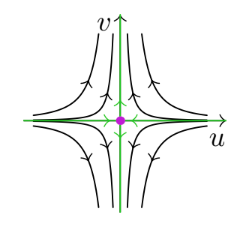
\includegraphics[scale=0.5]{images/sedlo.png}}
    \caption{Седло}
\end{figure}

\noindent \textbf{Случай $\lambda_1 = \lambda_2$}

Если геометрическая кратность собственного числа $\lambda = \lambda_{1,2}$ равна двум, то $A = diag(\lambda, \lambda)$. Тогда решения системы $x = C_1e^{\lambda t}$, $y = C_2e^{\lambda t}$. Исключая отсюда параметр $t$ получаем, что фазовые траектории --- лучи, входящие в начало координат при $\lambda < 0$, и выходящие из него, если $\lambda > 0$. Соответствующая точка покоя --- устойчивый или неустойчивый \textbf{дикритический узел} (см. \hyperref[dikrit]{рисунок}).

\begin{figure}[H]\label{dikrit}
    \center{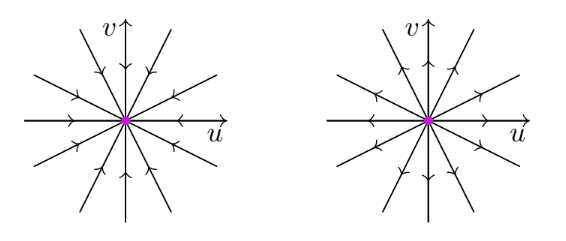
\includegraphics[scale=0.5]{images/dikrit.png}}
    \caption{Устойчивый и неустойчивый дикритический узел}
\end{figure}

Пусть собственное число $\lambda$ имеет геометрическую кратность $1$. Подставляя в систему $r = Ts$, где $T$ --- матрица перехода к жорданову базису, получаем
\begin{equation*}
    \dot{s} =
    \begin{pmatrix}
        \lambda & 1       \\
        0       & \lambda
    \end{pmatrix}
    s
\end{equation*}
Тогда
\begin{equation*}
    s = C_1e^{\lambda t}
    \begin{pmatrix}
        1 \\
        0
    \end{pmatrix}
    + C_2e^{\lambda t} (t
    \begin{pmatrix}
        1 \\
        0
    \end{pmatrix}
    +
    \begin{pmatrix}
        0 \\
        1
    \end{pmatrix}
    )
\end{equation*}
Следовательно, $u = C_1e^{\lambda t} + C_2te^{\lambda t}$, $v = C_2e^{\lambda t}$.

Заметим, что одновременная замена знака у постоянных $C_1$ и $C_2$ переводит фазовую траекторию в симметричную ей относительно начала координат. При $C_1 \neq 0$, $C_2 = 0$ функции $u$ и $v$ определяют полуоси координатной оси $u$. Таким образом, достаточно изучить фазовый портрет при $v > 0$.

Выражая параметр $t$ через $v$ и подставляя его в выражение для $u$, находим уравнение траекторий
\begin{equation*}
    u = Cv + \frac{\ln{v}}{\lambda}v
\end{equation*}
где $C = \frac{C_1}{C_2}$. Производная $u'_v$ указывает на то, что все фазовые траектории касаются оси $u$ при $v \to 0$ (см. \hyperref[virozhd]{рисунок}). Соответствующая точка покоя --- \textbf{вырожденный узел} (устойчивый при $\lambda < 0$ и неустойчивый при $\lambda > 0$).

\begin{figure}[H]\label{virozhd}
    \center{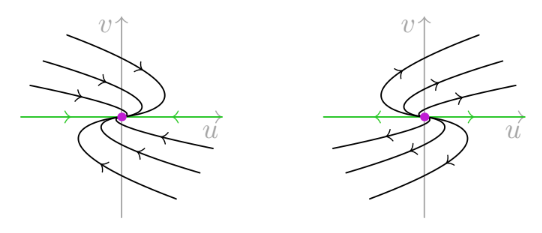
\includegraphics[scale=0.5]{images/virozhd.png}}
    \caption{Устойчивый и неустойчивый вырожденный узел}
\end{figure}

\subsection*{23. Классификация точек покоя ЛОС 2-го порядка (случай комплексных корней).}

Исследуем подробно поведение траекторий в окрестности точки покоя линейной системы
\begin{equation*}
    \dot{r} = Ar
\end{equation*}
если $A \in M_2(\mathbb{R})$. Пусть $\det A \neq 0$, тогда имеется единственное положение равновесия $r = 0$ и собственные числа $\lambda_1, \lambda_2$ матрицы $A$ отличны от нуля.\\

\noindent \textbf{Случай $\lambda_1, \lambda_2 \in \mathbb{C}$, $Im\, \lambda_{1,2} \neq 0$}

Поскольку матрица $A$ вещественная, то $\lambda_1 = \overline{\lambda_2}$. Пусть $\lambda = \lambda_1$, $h$ --- соответствующий собственный вектор. Тогда $Re\, h$, $Im\, h$ --- базис в $\mathbb{R}^2$. Поскольку
\begin{equation*}
    Re\, h = \frac{h + \overline{h}}{2}, \quad Im\, h = \frac{h - \overline{h}}{2i} = \frac{-ih + i\overline{h}}{2}
\end{equation*}
то матрица перехода $T$ к базису $Re\, h$, $Im\, h$ представима в виде
\begin{equation*}
    T = (Re\, h, Im\, h) = \frac{1}{2}(h,\overline{h})
    \begin{pmatrix}
        1 & -i \\
        1 & i
    \end{pmatrix}
\end{equation*}

Пусть $H = (h, \overline{h})$ --- матрица перехода к собственному базису. Подставляя $r = Ts$ в уравнение $\dot{r} = Ar$, находим
\begin{equation*}
    \frac{1}{2}H
    \begin{pmatrix}
        1 & -1 \\
        1 & i
    \end{pmatrix}
    \dot{s} = A\frac{1}{2}H
    \begin{pmatrix}
        1 & -1 \\
        1 & i
    \end{pmatrix}
    s
\end{equation*}
Сокращая на множитель $\frac{1}{2}$ и умножая слева на $H^{-1}$, получаем
\begin{equation}
    \begin{pmatrix}
        1 & -1 \\
        1 & i
    \end{pmatrix}
    \dot{s} = H^{-1}AH
    \begin{pmatrix}
        1 & -1 \\
        1 & i
    \end{pmatrix}
    s \label{newsyst2}
\end{equation}
Поскольку $H^{-1}AH = diag(\lambda, \overline{\lambda})$, то система \eqref{newsyst2} имеет вид
\begin{equation*}
    \begin{cases}
        \dot{u} - i\dot{v} = \lambda(u - iv) \\
        \dot{u} + i\dot{v} = \overline{\lambda}(u + iv)
    \end{cases}
\end{equation*}

Уравнения этой системы равносильны: одно получается из другого при комплексном сопряжении. Поэтому достаточно рассмотреть только одно из них. Положим $z = u + iv$. Тогда второе уравнение принимает вид
\begin{equation*}
    \dot{z} = \overline{\lambda}z
\end{equation*}
Его решения $z = Ce^{\overline{\lambda}t}$

Пусть $\lambda = \alpha + i\beta$, $C = ae^{i\varphi}$. Тогда
\begin{equation*}
    z = ae^{\alpha t}e^{i(\varphi - \beta t)}
\end{equation*}

При $\alpha = 0$ получаем окружности радиуса $a$. Соответствующая устойчивая, но не асимптотически устойчивая точка покоя называется \textbf{центр}. Направление обхода окружностей зависит от знака $\beta$.

При $\alpha > 0$ получаем логарифмическую спираль. Модуль $z$ возрастает, значит, точка удаляется от начала координат, при этом совершая вокруг него обороты. Данное положение равновесия называется \textbf{неустойчивый фокус}.

При $\alpha < 0$ спираль закручивается. Точка покоя --- \textbf{устойчивый фокус}. Направление закручивания или раскручивания траекторий в случае фокуса зависит от знака $\beta$ (см. \hyperref[focus]{рисунок}).

\begin{figure}[H]\label{focus}
    \center{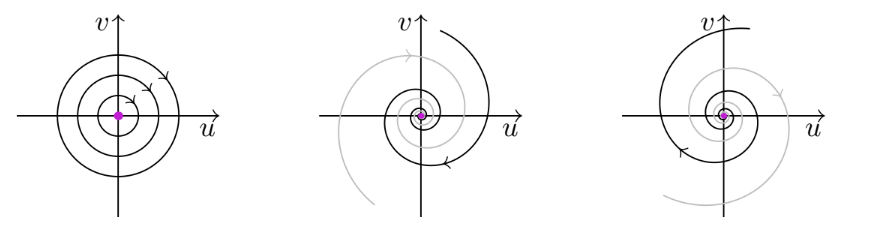
\includegraphics[scale=0.5]{images/focus.png}}
    \caption{Центр, устойчивый и неустойчивый фокус}
\end{figure}

\subsection*{24. Теорема Ляпунова об устойчивости.}

Рассмотрим нелинейную автономную систему $\dot{r} = f(r)$. Допустим, вектор-функция $f$ дифференцируема. Тогда по формуле Тейлора
\begin{equation*}
    f(r) = f(0) + f'(0)r + o(r)
\end{equation*}

\noindent \textbf{Определение.} Пусть $f(0) = 0$. Тогда система
\begin{equation*}
    \dot{r} = f'(0)r
\end{equation*}
называется \textbf{системой первого приближения} или \textbf{линеаризацией} системы $\dot{r} = f(r)$\\

\noindent \textbf{Теорема (Ляпунов, устойчивость по первому приближению).} Пусть $f \in C^2(\Omega)$, где $\Omega \subset \mathbb{R}^n$ --- окрестность нуля, $f(0) = 0$. Тогда нулевое решение системы $\dot{r} = f(r)$
\begin{enumerate}
    \item асимптотически устойчиво, если $Re\, \lambda < 0$ для любого $\lambda \in spec\, f'(0)$
    \item неустойчиво, если найдется $\lambda \in spec\, f'(0)$, для которого $Re\, \lambda > 0$
\end{enumerate}

\noindent \textbf{Доказательство.} В окрестности $r = 0$ систему $\dot{r} = f(r)$ можно записать в виде
\begin{equation*}
    \dot{r} = Ar + q(r)
\end{equation*}
где $q(r) = o(|r|)$ при $|r| \to 0$. Решение задачи Коши $\dot{r} = f(r),\, r(0) = r_0$ в силу предположения в некоторой окрестности $r_0$ определено для всех $t > 0$. Его можно записать в виде
\begin{equation*}
    r(t) = e^{At}\cdot r_0 + \int_0^t e^{A(t-\tau)}\cdot q(r(\tau))d\tau
\end{equation*}

Если $Re\, \lambda < 0$ для любого $\lambda \in spec\, f'(0)$, то найдется $\mu > 0$ такое, что $Re\, \lambda < -2\mu < 0$. Решение задачи Коши для $\dot{r} = Ar,\, r(0) = r_0$ имеет вид
\begin{equation*}
    r = e^{At}\cdot r_0
\end{equation*}

Покажем, что найдется такое $M > 0$, что норма матричной экспоненты
\begin{equation*}
    |e^{At}| \le Me^{-\mu t}, \quad \forall t \ge 0
\end{equation*}
Каждый элемент $a_{ij}(t)$ матрицы $e^{At}$ является конечной суммой квазимногочленов
\begin{equation*}
    a_{ij}(t) = \sum_{k=1}^m P_k^{(i,j)}(t) e^{\lambda_kt}
\end{equation*}
где $P_k^{(i,j)}(t)$ --- многочлены, $m$ --- количество собственных чисел. Всегда найдется такое число $c_{ij} > 0$, что для всех $k \in [1:m]$
\begin{equation*}
    |P_k^{(i,j)}(t)e^{\lambda_kt}| \le c_{ij}e^{-\mu t}, \quad \forall t > 0
\end{equation*}
Тогда
\begin{equation*}
    \begin{aligned}
         & |r(t)| \le |e^{At}| |r_0| = |r_0| \sqrt{\sum_{i,j=1}^n |a_{ij}(t)|^2} \le  \\
         & \le |r_0| e^{-\mu t}m \sqrt{\sum_{i,j=1}^n |c_{ij}|^2} = Me^{-\mu t} |r_0|
    \end{aligned}
\end{equation*}

Так как $q(r) = o(|r|)$ при $|r| \to 0$, то для любого $\varepsilon > 0$ найдется $\delta = \delta(\varepsilon) > 0$ такое, что из $|r| < \delta$ следует $|q(r)| \le \varepsilon|r|$. Тогда при всех $t > 0$
\begin{equation*}
    \begin{aligned}
        |r(t)| & \le |e^{At} r_0| + \int_0^t |e^{A(t - \tau)} q(r(\tau))|d\tau \le               \\
               & \le |e^{At}| |r_0| + \int_0^t |e^{A(t - \tau)}| |q(r(\tau))|d\tau \le           \\
               & \le Me^{-\mu t} |r_0| + \varepsilon M\int_0^t e^{-\mu (t - \tau)}|r(\tau)|d\tau
    \end{aligned}
\end{equation*}

Если положить $u(t) = e^{\mu t}|r(t)|$, то отсюда находим, что
\begin{equation*}
    u(t) \le M |r_0| + \varepsilon M\int_0^t u(\tau)d\tau
\end{equation*}
Функция $u(t)$ удовлетворяет условиям леммы Гронуолла. Значит, что при всех $t > 0$
\begin{equation*}
    u(t) \le M |r_0|e^{\varepsilon Mt}
\end{equation*}
Заменяя $u(t)$ на $e^{\mu t} |r(t)|$, получаем оценку
\begin{equation*}
    |r(t)| \le M |r_0|e^{-(\mu - \varepsilon M)t}
\end{equation*}
Из полученной оценки следует, что при достаточно малых $\varepsilon > 0$
\begin{equation*}
    r(t) \to 0, \quad t \to +\infty
\end{equation*}
если фиксировать $\varepsilon > 0$, положив, например, $\varepsilon = \frac{\mu}{2M}$. Кроме того, взяв $\delta = \delta(\varepsilon) = \frac{\varepsilon}{M}$, из оценки получаем, что $|r(t)| < \varepsilon$ при $|r_0| < \delta$ для всех $t > 0$.

Второй пункт теоремы следует непосредственно из доказательства теоремы об устойчивости ЛОС с постоянными коэффициентами (мб кукарек, хз как доказать).\\

\noindent \textbf{Определение.} Пусть $\Omega \subset \mathbb{R}^n$ --- окрестность нуля. Функция $V \in C^1(\Omega)$ называется \textbf{функцией Ляпунова} системы $\dot{r} = f(r)$, если
\begin{itemize}
    \item $V(r) > 0$ при всех $r \in \Omega \setminus \{0\}$, $V(0) = 0$
    \item $V' \cdot f \le 0$ при всех $r \in \Omega$
\end{itemize}

\noindent \textbf{Теорема (Ляпунов, об устойчивости).} Пусть $f \in Lip_{loc}(\Omega)$, $\Omega \subset \mathbb{R}^n$ --- окрестность нуля, $f(0) = 0$. Если в области $\Omega$ существует функция Ляпунова системы $\dot{r} = f(r)$, то $r = 0$ --- устойчивое решение.\\

\noindent \textbf{Доказательство.} Будем доказывать от противного. Пусть нулевое положение равновесия неустойчиво. Тогда найдется такое $\varepsilon > 0$, что при любом сколь угодно малом $\delta > 0$ можно выбрать такое начальное положение $r_0$ из $\delta$-окрестности нуля, что будет ложным утверждение
\begin{equation}
    \forall t \ge 0 \quad |r(t, 0, r_0)| < \varepsilon \label{lyap}
\end{equation}
Все числа, меньшие $\varepsilon$, обладают тем же свойством, что и $\varepsilon$. Поэтому можно считать, что $\varepsilon$-окрестность содержится вместе с границей в области $\Omega$.

Ложность утверждения \eqref{lyap} означает одно из двух:
\begin{enumerate}
    \item решение $r(t, 0, r_0)$ определено не при всех $t \ge 0$
    \item найдется $t_{\varepsilon} > 0$, такое что $|r(t_{\varepsilon}, 0, r_0)| \ge \varepsilon$
\end{enumerate}

Допустим, выполнено (1), то есть максимальное решение $r(t, 0, r_0)$ (которое существует и единственно) определено на интервале $(a,b) \ni 0$, где $b < +\infty$. Построим параллелепипед $[0,b] \times \overline{B}_{\varepsilon}(0)$, где $\overline{B}_{\varepsilon}(0)$ --- замыкание $\varepsilon$-окрестности нуля. Интегральная кривая решения $r(t, 0, r_0)$ выйдет на его границу при некотором $t_{\varepsilon} < b$. Значит, верно утверждение (2).

Итак, достаточно получить противоречие, если верно (2). Будем считать, что $t_{\varepsilon}$ --- это точка, в которой $r(t_{\varepsilon}, 0, r_0) \in \partial B_{\varepsilon}(0)$, где $\partial B_{\varepsilon}(0)$ --- граница $\varepsilon$-окрестности нуля.

Пусть $V_M = \displaystyle\min_{r \in \partial B_{\varepsilon}(0)}V(r)$. Поскольку $V(r) \to 0$ при $r \to 0$, то можно выбрать $\delta$ так, чтобы $V(r) < \frac{V_M}{2}$ при $|r| < \delta$. Положим
\begin{equation*}
    v(t) = V(r(t, 0, r_0))
\end{equation*}
где $r_0$ выбрано из $\delta$-окрестности нуля так, чтобы выполнялось (2).

Функция $v$ дифференцируема
\begin{equation*}
    \begin{aligned}
         & v(0) = V(r_0) < \frac{V_M}{2}                              \\
         & v(t_{\varepsilon}) = V(r(t_{\varepsilon}, 0, r_0)) \ge V_M
    \end{aligned}
\end{equation*}
Поэтому найдется точка $t_1 \in (0, t_{\varepsilon})$, в которой $\dot{v}(t_1) > 0$.

Однако, исходя из второго свойства функции Ляпунова, имеем
\begin{equation*}
    \dot{v}(t_1) = V'(r(t_1, 0, r_0))\cdot r'_t(t_1, 0, r_0) = V'(r(t_1, 0, r_0)) \cdot f(r(t_1, 0, r_0)) \le 0
\end{equation*}
Полученное противоречие завершает доказательство теоремы.\\

\noindent \textbf{Теорема (Ляпунов, об асимптотической устойчивости).} Если в условиях предыдущей теоремы выполнено $V' \cdot f < 0$ в области $\Omega \setminus \{0\}$, то нулевое решение системы $\dot{r} = f(r)$ асимптотически устойчиво.


\section*{Дополнительные вопросы}

\subsection*{Уравнение 1-го порядка и его решение.}

% \begin{definition}
Это уравнение вида \(F(x, y, y') = 0\).
% \end{definition}
% \begin{definition}
Функция \(\varphi\) --- решение такого дифференциального уравнения, если:
\begin{enumerate}
    \item \(\varphi\in C^1(a, b)\)
    \item \(F(x, \varphi(x), \varphi'(x)) \equiv 0\) на \((a, b)\)
\end{enumerate}
% \end{definition}
\begin{example}
    \(y' - x = 0\), решение \(y = \frac{x^2}{2} + C\).
\end{example}

Методов решения много, все относятся к частным случаям.

\subsection*{Интегральная кривая уравнения.}

Это график решения уравнения.

\subsection*{Общее решение уравнения.}

Это множество всех его решений.

\subsection*{Уравнение 1-го порядка, разрешённое относительно производной. Геометрический смысл.}

Это уравнение вида \(y' = f(x, y)\).

Пусть \(\varphi\) решение этого уравнения. Тогда \(\varphi'(x) = f(x, \varphi(x))\), то есть тангенс угла наклона касательной к интегральной кривой в точке \((x_0, y_0)\) это \(f(x_0, y_0)\)

\subsection*{Ломаная Эйлера.}

См. 4

\subsection*{Уравнение в дифференциалах, его решение и параметрическое решение.}

Уравнение в дифференциалах получается, если в уравнении, разрешенном относительно производной, записать \(y' = \frac{dy}{dx} \):
\[P(x, y) dx + Q(x, y) dy = 0\]

Функция \(\varphi\) --- решение такого дифференциального уравнения, если:
\begin{enumerate}
    \item \(\varphi\in C^1(a, b)\)
    \item \(P(x, \varphi(x)) + Q(x, \varphi(x)) \varphi'(x) \equiv 0\) на \((a, b)\)
\end{enumerate}

Аналогично можно определить решение вида \(x = \psi(y)\).

Функция \(r = (\varphi(t), \psi(t))\) --- \textbf{параметрическое} решение такого уравнения на \(\alpha, \beta\), если:
\begin{enumerate}
    \item \(\varphi, \psi\in C^{1}(\alpha, \beta)\) и \(r'(t)\neq 0\) на \(t\in (\alpha, \beta)\)
    \item \(P(\varphi(t), \psi(t)) + Q(\varphi(t), \psi(t))\psi'(t) \equiv 0\) на \(t\in (\alpha, \beta)\)
\end{enumerate}

\begin{example}
    \[xdx + ydy = 0\]

    Подстановкой тривиально можно убедиться, что \(y = \sqrt{C^2 - x^2}\) --- решение этого уравнения.

    Параметрическое решение \((C\cos t, C\sin t)\)
\end{example}

\subsection*{Особые точки уравнения в дифференциалах.}

\((x_0, y_0)\) --- особая, если \(P(x_0, y_0) = Q(x_0, y_0) = 0\)

\begin{example}
    \[xdx + ydy = 0\]

    Особая точка \((0, 0)\), через нее ничто не проходит.
\end{example}

\subsection*{Геометрический смысл уравнения в дифференциалах и его решения.}

Пусть \(r = (x(t), y(t))\) есть параметрическое решение уравнения на \((\alpha, \beta)\). Тогда при \(t\in(\alpha, \beta)\):
\[P(x(t), y(t))x'(t) + Q(x(t), y(t))y'(t) = 0\]
\[F(r(t))r'(t) = 0\]
Таким образом, любая интегральная кривая в каждой своей точке перпендикулярная вектору \(F(x, y)\)

\subsection*{Задача Коши (ЗК) для уравнения 1-го порядка, разрешённого относительно производной.}

Задача Коши --- задача поиска решения уравнения, удовлетворяющему \(y(x_0) = y_0\).

\begin{theorem}
    \(G\subset\R^2\) --- область, \(f\in C(G), (x_0, y_0)\in G\). Тогда в некоторой окрестности \(x_0\) существует решение задачи Коши.
\end{theorem}
\begin{theorem}
    Как в предыдущей теореме, но \(f'_y\in C(G)\). Тогда решение задачи Коши единственно.
\end{theorem}

Таким образом, может быть такое, что в некоторых \textit{(или всех)} точках решение не единственно.

\subsection*{Особое решение уравнения.}

Это решение уравнения, в каждой точке которого нарушается локальная единственность решения задачи Коши.

\begin{example}
    \[y' = \sqrt[3]{y^2}\]
    Тогда особое решение \(y' \equiv 0\), его в любой точке \((x_0, 0)\) пересекает решение вида \(y = (x - x_0)^3 / 3\)
\end{example}

\subsection*{Однородное уравнение.}

Функция однородна степени \(\alpha\), если \(\forall t,x,y \ \ F(tx, ty) = t^\alpha F(x, y)\)

Однородное уравнение --- уравнение вида
\[P(x, y)dx + Q(x, y)dy = 0\]
, где \(P\) и \(Q\) однородные функции одной степени.

Замена \(z = \frac{y}{x}\) сводит это уравнение к уравнению с разделяющимися переменными.

\subsection*{Геометрическое свойство решений однородного уравнения.}

Пусть \(x = \varphi(t), y = \psi(t)\) --- параметрическое решение однородного дифура. Растянем пространство в \(\lambda\) раз, получим \(x = \lambda \varphi(t), y = \lambda \psi(t)\). При подстановке получим:
\[P(\lambda\varphi, \lambda\psi) \lambda\varphi' + Q(\lambda\varphi, \lambda\psi)\lambda\psi' = 0\]
По однородности:
\[P(\varphi, psi) \varphi' + Q(\varphi, \psi)\psi' = 0\]

Таким образом, любое растяжение \textit{(или сжатие)} решения однородного уравнения приводит к другому решению однородного уравнения.

\subsection*{Уравнение Бернулли.}

Это уравнение вида
\[y' = p(x) y + q(x) y^\alpha, \alpha\in\R\setminus \{0,1\}\]

Поделив на \(y^\alpha\) и заменив \(z = y^{1 - \alpha}\), получаем линейное.

\subsection*{Уравнение Риккати.}

\[y' = p(x) y^2 + q(x)y + r(x)\]

Оно решается только в особых случаях \textit{(например, \(\alpha = 2\))}, но если нашел какое-то решение \(\varphi\), то замена \(y = z + \varphi\) сводит к Бернулли.

\subsection*{Уравнение в полных дифференциалах.}

Это уравнение вида
\[P(x, y) dx + Q(x, y)dy = 0\]
, при этом
\[\exists u : du = P(x, y) dx + Q(x, y) dy\]

Решение имеет вид \(u(x, y) = C\)

Обязательное условие на существование \(u\) это \(P'_y = Q'_x\). Если при этом \(P, Q\in C^1(G)\) и \(G\) односвязна, то это условие еще и достаточно.

Если область прямоугольная, то можно решить систему \(\begin{cases}
    u_x' = P \\
    u_y' = Q
\end{cases}\) следующим образом: Решаем первое уравнение при фиксированном \(y\), после чего заменяем \(C = C(y)\) и находим \(C\) как функцию.

В таком случае \(u\) есть потенциал векторного поля \((P, Q)\).

\subsection*{Интегрирующий множитель.}

Это то, на что мы домножаем уравнение, чтобы получить уравнение в полных дифференциалах.

Если \(\mu\) --- инт. множитель, то
\[(\mu P)'_y = (\mu Q)'_x\]
, то есть
\[\mu'_y P - \mu'_x Q = (Q'_x - P'_y) \mu\]

Это сложно решить, но иногда решается при \(\mu'_x \equiv 0\) или \(\mu'_y \equiv 0\).

\subsection*{Уравнение n-го порядка и его решение.}

Это уравнение вида:
\[F(x, y, y', \dots , y^{(n)}) = 0\]

Его решение на \(a, b\) --- \(\varphi\), такое что:
\begin{enumerate}
    \item \(\varphi\in C^n(a, b)\)
    \item \(F(x, \varphi(x), \varphi'(x), \dots , \varphi^{(n)}(x)) \equiv 0\) на \((a, b)\)
\end{enumerate}

\subsection*{ЗК для уравнения, разрешённого относительно старшей производной.}

Это уравнение вида \(y^{(n)} = f(x, y, y', \dots , y^{(n - 1)})\).

Задача Коши для него имеет вид \(y(x_0) = y_0, y'(x_0) = y_1, \dots , y^{(n - 1)}(x_0) = y_{n - 1}\)

\subsection*{Методы понижения порядка уравнения.}

\begin{itemize}
    \item \(y^{(n)} = f(x) \implies y^{(n - 1)} = \int f(x) dx\)
    \item \(F(x, y^{(k)}, y^{(k + 1)}, \dots , y^{(n)}) \xRightarrow{z = y^{(k)}} F(x, z, \dots z^{(n - k)}) = 0\)
    \item \(F(y, y', \dots , y^{(n)}) = 0\). Тогда пусть \(z = y'\), \(y''_{xx} = z'_y z, y'''_{x x x} = z''_{yy} z^2 + z'_y{^2} z\) и т.д.
    \item Пусть \(F\) линейна по \(y\). Тога можно заменить \(z = y'/y\)
    \item \(F(x, y, y', \dots , y^{(n)}) = \cfrac{d}{dx} \Phi(x, y, y', \dots , y^{(n - 1)}) \Rightarrow \Phi(x, y, y', \dots , y^{(n - 1)}) = C\)
\end{itemize}

\subsection*{Нормальная система уравнений, её решение.}

Нормальная система порядка \(n\) это система вида:
\[\begin{cases}
        \dot{x}_1 = f_1(t, x_1, \dots x_n) \\
        \vdots                             \\
        \dot{x}_n = f_n(t, x_1, \dots x_n) \\
    \end{cases}\]

Можно ввести пару обозначений для краткости:
\[r = \begin{pmatrix} x_1 \\ \vdots \\ x_n \end{pmatrix} \quad f(t, r) = \begin{pmatrix} f_1(t, r) \\ \vdots \\ f_n(t, r) \end{pmatrix} \quad \dot{r} = f(t, r)\]

\(\varphi\) --- решение такой системы, если:
\begin{enumerate}
    \item \(\varphi \in C^1((a, b) \to \R^n)\)
    \item \(\dot \varphi(t) \equiv f(t, \varphi(t))\) на \((a, b)\)
\end{enumerate}

\subsection*{Интегральная кривая нормальной системы.}

Это график решения, но теперь он в \((n + 1)\)-мерном пространстве.

\subsection*{Глобальное и локальное условие Липшица.}

Функция \(f : \R^m \to \R^n\) удовлетворяет условию Липшица на множестве \(D\), если \(\exists L\) --- константа Липшица, что для \(\forall r_1, r_2\in D \ \ |f(r_2) - f(r_1)| \leq L|r_2 - r_1|\)

\begin{example}
    Пусть \(f(x) = \sqrt{x}\). Тогда \(f\in \text{Lip}[1 / 2, 1], f\not\in \text{Lip}(0, 1], f\in \text{Lip}_{loc}(0, 1]\)
\end{example}

Функция \(f : \R^{n + 1}_{t, r} \to \R^n\) удовлетворяет условию Липшица по \(r\) \textit{(равномерно по \(t\))} на множестве \(D\), если \(\exists L\), что для \(\forall (t, r_1), (t, r_2)\in D \ \ |f(t, r_2) - f(t, r_1)| \leq L|r_2 - r_1|\), обозначается \(f\in \text{Lip}_r(D)\)

\(f \in \text{Lip}_{loc}(D)\) локально, если \(\forall x_0\in D \ \ \exists U(x_0) \ \ f\in \text{Lip}(U(x_0))\)

\subsection*{Приближения Пикара.}

\begin{itemize}
    \item \(\varphi_0(t) = 0\)
    \item \(\varphi_{k + 1}(t) = \int_0^t f(\tau, \varphi_k(\tau))d\tau\)
\end{itemize}

\subsection*{Сведение уравнения n-го порядка к равносильной системе.}

Пусть \(\Lambda_n y = (y, \dot{y}, \dots , y^{(n - 1)})^T\)

\begin{lemma}
    \(y\) --- решение \(y^{(n)} = f(t, y, \dot{y}, \dots , y^{(n - 1)})\) на \((a, b)\) \(\Leftrightarrow\) \(\Lambda_n y\) --- решение на \((a, b)\) \[\begin{pmatrix} \dot{y}_1 \\ \vdots \\ \dot{y}_{n - 1} \\ \dot{y}_{n} \end{pmatrix} = \begin{pmatrix} y_2 \\ \vdots \\ y_n \\ f(t, y_1, \dots , y_n) \end{pmatrix} \]
\end{lemma}
\begin{proof}\itemfix
    \begin{itemize}
        \item [\( \Rightarrow \)] Пусть \(y\) --- решение первого уравнения. Тогда пусть \(y_k = y^{(k - 1)}\). Тогда первые \(n - 1\) уравнений решаются, а \(\dot{y}_n = y^{(n)} = f(t, y, \dot{y}, \dots , y^{(n - 1)})\), искомое верно.
        \item [\( \Leftarrow \)] Пусть \(r\) --- решение второго уравнения. Будем последовательно дифференцировать первое уравнение и получим искомое.
    \end{itemize}
\end{proof}

\subsection*{Максимальное решение.}

Решение \(\varphi\) продолжимо, если есть решение \(\psi\) на большем отрезке, равное \(\varphi\) на \(\text{dom} \varphi\).

Если у решения нет продолжения, оно максимально.

\subsection*{Определитель Вронского (решений ЛОС и ЛОУ) и его свойства.}

Вронскиан множества вектор-фукнций \(\{r_k\}_{k = 1}^n\), где \(r_k = (x_{k1}, x_{k2}, \dots, x_{kn})^T\):
\[W(t) = \det (r_1(t), \dots , r_n(t)) = \begin{vmatrix} x_{11}(t) & x_{21}(t) & \dots & x_{n1}(t) \\ x_{12}(t) & x_{22}(t) & \dots & x_{n2}(t) \\ \vdots & \vdots & \ddots & \vdots \\ x_{1n}(t) & x_{2n}(t) & \dots & x_{nn}(t) \end{vmatrix} \]

\noindent \textbf{Определение.} \textbf{Определителем Вронского} (или \textbf{вронскианом}) функций $y_1, y_2, \ldots, y_n \in C^{n-1}(a,b)$ называют
\begin{equation*}
    W(t) = \begin{vmatrix}
        y_1(t)         & y_2(t)         & \ldots & y_n(t)         \\
        \dot{y}_1(t)   & \dot{y}_2(t)   & \ldots & \dot{y}_n(t)   \\
        \ldots                                                    \\
        y_1^{(n-1)}(t) & y_2^{(n-1)}(t) & \ldots & y_n^{(n-1)}(t)
    \end{vmatrix}
\end{equation*}

\subsection*{Фундаментальная система решений.}

\noindent \textbf{Определение.} \textbf{Фундаментальной системой решений} системы уравнений $\dot{r} = P(t)r$ называется совокупность ее $n$ линейно независимых решений.

\subsection*{Фундаментальная матрица.}

\noindent \textbf{Определение.} \textbf{Фундаментальная матрица системы} $\dot{r} = P(t)r$ --- матрица, столбцы которой образуют фундаментальную систему решений.

\subsection*{Метод неопределённых коэффициентов для ЛС.}

\(A\in M_n(\mathbb{C}), k\in \Z_{+}, a_j\in\mathbb{C}^n\) при \(j\in[0,k]\cap \Z, \gamma\in\mathbb{C}\), \(p_k(t)\) --- многочлен от \(t\) степени \(k\), при этом коэфы \(a_j\).

Тогда \(e^{\gamma t} q_{k + s}(t)\) есть решение системы \(\dot{r} = Ar + e^{\gamma t} p_k(t)\), где \(q_{k + s}(t)\) --- вектор-многочлен степени \( \leq k + s\), и \(s\):
\begin{enumerate}
    \item \( = 0\), если \(\lambda\) не СЗ \(A\)
    \item \( =\) максимальный размер жордановых клеток, соответствующих \(\gamma\)
\end{enumerate}

\subsection*{Характеристический многочлен ЛУ.}

В дальнейшем для краткости используется обозначение
\begin{equation*}
    Ly = \frac{d^n}{dt^n}y + a_{n-1}\frac{d^{n-1}}{dt^{n-1}}y + \ldots + a_1\frac{d}{dt}y + a_0y = \left(\sum_{k = 0}^n a_k\frac{d^k}{dt^k} \right)y
\end{equation*}
где $a_n = 1$. При помощи оператора $L$ уравнение \eqref{lupost} записывается в виде
\begin{equation*}
    Ly = f(t)
\end{equation*}

Рассмотрим линейное однородное уравнение
\begin{equation}
    Ly = 0 \label{lodnpost}
\end{equation}
Применяя оператор $L$ к функции $e^{\lambda t}$, находим
\begin{equation*}
    L(e^{\lambda t}) = \sum_{k = 0}^n a_k\frac{d^k}{dt^k}e^{\lambda t} = \left(\sum_{k = 0}^n a_k\lambda^k \right)e^{\lambda t}
\end{equation*}

\noindent \textbf{Определение.} Многочлен
\begin{equation*}
    p(\lambda) = \lambda^n + a_{n-1}\lambda^{n-1} + \ldots + a_1\lambda + a_0
\end{equation*}
называется \textbf{характеристическим многочленом} уравнения \eqref{lupost}, а его корни --- \textbf{характеристическими числами} уравнения \eqref{lupost}.

\subsection*{Метод неопределённых коэффициентов для ЛУ.}

Пусть в уравнении
\[y^{(n)} + a_{n - 1}y^{(n - 1)} + \dots + a_1 \dot{y} + a_0 y = f(t)\]
\(f(t) = p_k (t) e^{\gamma t}\), где \(p_k(t)\) --- многочлен \textit{(\(f\) --- квазимногочлен)}. Тогда у этого уравнения есть единственное частное решение вида
\[\varphi(t) = t^m q_k(t) e^{\gamma t}\]
, где \(q_k\) --- многочлен степени \(k\), при этом \(m\):
\begin{enumerate}
    \item \( = 0\), если \(\gamma\) --- не характеристическое число
    \item \( = \) кратность \(\gamma\) как хар. числа.
\end{enumerate}

\subsection*{Автономная система.}

Это система вида
\[\dot{r} = f(r)\]

\subsection*{Фазовое пространство автономной системы. Фазовая траектория, фазовый портрет, фазовая скорость, точка покоя.}

\begin{itemize}
    \item Фазовое пространство --- \(\text{dom} f\)
    \item Расширенное фазовое пространство --- \(\R \times \text{dom} f\)
    \item Фазовая траектория --- проекция интегральной кривой на фазовое пространство параллельно оси времени
    \item Фазовый портрет --- совокупность фазовых траекторий
    \item Фазовая сокрость в точке \(r\) --- \(f(r)\)
\end{itemize}

\subsection*{Устойчивость по Ляпунову и ассимптотическая устойчивость.}

\noindent \textbf{Определение.} Положение равновесия $r = 0$ автономной системы $\dot{r} = f(r)$ называется \textbf{усточивым (по Ляпунову)}, если для любой $\varepsilon$-окрестности нуля найдется такая $\delta$-окрестность нуля, что любое решение, выходящее из этой $\delta$-окрестности, во все будущие моменты времени отличается от нуля менее, чем на $\varepsilon$. То есть
\begin{equation*}
    \forall \varepsilon > 0 \, \exists \delta > 0:\, |r_0| < \delta \implies \forall t \ge 0 \, |r(t,0,r_0)| < \varepsilon
\end{equation*}
В противном случае положение равновесия называется \textbf{неустойчивым}.\\

\noindent \textbf{Определение.} Положение равновесия $r = 0$ автономной системы $\dot{r} = f(r)$ называется \textbf{асимптотически устойчивым}, если
\begin{itemize}
    \item $r = 0$ устойчиво
    \item все решения, начинающиеся в некоторой окрестности нуля, в будущем стремятся к нулю, то есть
          \begin{equation*}
              \exists \delta > 0:\, |r_0| < \delta \implies r(t,0,r_0) \to 0\, \text{при } t \to +\infty
          \end{equation*}
\end{itemize}

\subsection*{Функция Ляпунова.}

\noindent \textbf{Определение.} Пусть $\Omega \subset \mathbb{R}^n$ --- окрестность нуля. Функция $V \in C^1(\Omega)$ называется \textbf{функцией Ляпунова} системы $\dot{r} = f(r)$, если
\begin{itemize}
    \item $V(r) > 0$ при всех $r \in \Omega \setminus \{0\}$, $V(0) = 0$
    \item $V' \cdot f \le 0$ при всех $r \in \Omega$
\end{itemize}

\subsection*{Теорема об устойчивости по первому приближению.}

Есть система \(\dot{r} = f(r)\). Пусть \(f\) --- дифф. Тогда \(f(r) = f(0) + f'(0)r + o(r)\). Пусть \(f(0) = 0\) \textit{(если не так, пошафлим координаты)}. Тогда \(f(r) = f'(0)r\) есть сист��ма первого приближения.

\begin{theorem}
    \(f\in C^2(\Omega), \Omega\subset \R^n\) --- окретсность нуля, \(f(0) = 0\). Тогда нулевое решение системы \(\dot{r} = f(r)\):
    \begin{enumerate}
        \item Асимптотически устойчиво, если \(\Re \lambda < 0 \ \ \forall \lambda \in \text{spec} f'(0)\)
        \item Неустойчиво, если \(\exists \lambda\in \text{spec} f'(0) : \Re \lambda > 0\)
    \end{enumerate}
\end{theorem}


\end{document}
 